
\chapter{Applications of General Relativity}
\label{ch:GRapplications}


\section{Weak Gravitational Fields}
When we first derived Einstein’s equations, we checked that we were on the right track by
considering the Newtonian limit. This amounted to the requirements that the gravitational
field be weak, that it be static (no time derivatives), and that test particles be moving slowly.
In this section we will consider a less restrictive situation, in which the field is still weak but
it can vary with time, and there are no restrictions on the motion of test particles. This
will allow us to discuss phenomena which are absent or ambiguous in the Newtonian theory,
such as gravitational radiation (where the field varies with time) and the deflection of light
(which involves fast-moving particles).












\section{Gauge transformations in general relativity}
\subsection{Firstly, remark on the difference to diffeomorphism invariance, aka general covariance}
Gauge invariance is a property where a given field is generated by more than one potential. While a field is unique, the potential that generates it need not be.
The difference between gauge invariance and general covariance, aka diffeomorphism invariance is that the potential is a function of the coordinates, and it generates a field. The field is unique, but there may be many potentials that can generate it.\\
General covariance now is the ability to choose coordinates for general relativity as we like. This must be done carefully, utilizing symmetries and invariance arguments to make sure such transformations are allowable in specific situations.
\marginpar{ The laws of physics as we know them (standard model plus gravity) have gauge transformations that split into two separate, independent parts; transformations of the fields vs transformations of the coordinate system.  Supersymmetry uses a gauge transformation that combines coordinate and field transformations together.}
\\
\\
Equivalently formulated:\\
\begin{mybox}{Difference between gauge invariance and diffeomorphism invariance}
	\emph{A diffeomorphism is the same thing as a smooth coordinate transformation}, which is the same thing as saying that you can switch between two coordinate maps and \emph{leave the physical laws invariant}.\\ 
	There is also gauge invariance, which states that the laws (of physics, usually) remain invariant under a \emph{redefinition} of the fields (a transformation of the fields) that appear in the laws, e.g. in GR the field is $g\munu$ while in QED the field is redefined via a local $U(1)$ transformation as $\psi \rightarrow e^{i \alpha} \psi = \psi^\prime$.  However, coordinate transformations are equivalent to transformations of the fields (there's no difference between moving your coordinate frame to the left, by a metre, and moving all the fields to the right, by a metre, for example), so \emph{coordinate transformations are also a form of gauge transformations}.\\
	\\
	Note that forces arise from redefinitions - called \emph{local gauge transformations} - that vary in time and space.  The forces of the standard model of particle physics arise from local transformations of the fields.  Gravity arises from local coordinate invariance.
\end{mybox}
A gauge-invariant system is not just, as many people misconceive, a system with a local symmetry. Gauge symmetry isn’t really a symmetry in any case, it’s due to a redundancy in the system. Now we see that general relativity is an instance of a gauge-invariant theory too because since the theory does not care about my choice of coordinates, then it has such redundancies which are exactly the values of the coordinates in a chosen coordinate system. In “ordinary” 4-dimensional general relativity, I only need two local degrees of freedom to describe the physics of the theory, whereas the basic object that characterises gravity in the theory, namely the spacetime metric, naively has $10$ degrees of freedom; clearly there’s $8$ too many! Transformations among these redundant degrees of freedom are precisely implemented by diffeomorphisms in GR, consequently diffeomorphisms are the gauge “symmetry” of GR.


\subsection{On General Covariance and gauge symmetry by Weinberg}
As described in \ref{sec:generalcovariance}, General covariance is not an ordinary symmetry principle like Lorentz invariance, but is rather a dynamical principle that governs the effect of gravitational fields. As such, it bears a strong resemblance to another "dynamic symmetry", local gauge invariance, which governs the effects of electromagnetic fields. Local gauge invariance says that the differential equations satisfied by a set of charged fields $\psi(x)$ and the electromagnetic potential $A_\alpha(x)$ retain the same form when these fields are subjected to the transformations
\begin{equation}
\label{eq:EMgaugetrafo}
	\psi(x) \rightarrow \psi(x) e^{i e \varphi(x)}, \quad A_\alpha(x) \rightarrow A_{\alpha} (x) + \frac{\partial }{\partial x^\alpha} \varphi(x),
\end{equation}
thus the fields are transformed and not the coordinates as described above, where $e$ is the charge of the particle represented by $\psi$ and $\varphi(x)$ is an arbitrary function of the space-time coordinates $x^\alpha$. How are we to construct gauge-invariant equations ? Note that derivatives of a charged field $\psi$ do not behave under gauge transformations like $\psi$, but rather
\begin{equation}
	\frac{\partial}{\partial x^\alpha} \psi(x) \rightarrow \frac{\partial}{\partial x^\alpha }\left[\psi (x)e^{i e \varphi(x)} \right]=e^{ie\varphi(x)} \left[\frac{\partial \psi(x)}{\partial x^\alpha} + i e \psi(x) \frac{\partial \varphi(x)}{\partial x^\alpha}\right]
\end{equation}
just as derivatives of tensors do not behave like tensors under general coordinate transformations. It follows that an equation such as
\begin{equation}
	\left(\partial^2 - m^2\right) \psi(x) =0,\qquad \partial^2\equiv \eta^{\alpha  \beta} \frac{\partial}{\partial x^\alpha} \frac{\partial}{\partial x^\beta}
\end{equation}
is \emph{not} gauge-invariant, just as it is not generally covariant. Also note that the electromagnetic potential $A_\mu(x)$ obeys the inhomogeneous transformation law, just as the affine connection coefficients $\Gamma^\alpha\munu$ obeys the inhomogeneous transformation law \ref{eq:christoffelTrafo} for general coordinate transformations. In tensor analysis we put together derivatives of tensors and the affine connection coefficients $\Gamma$ to form "covariant derivatives" that transform like tensors. In electrodynamics we put together derivatives of fields and the vector potential to form "gauge-covariant derivatives"
\begin{equation}
	D_\alpha \psi(x) \equiv \left[\frac{\partial}{\partial x^\alpha} - i e A_\alpha(x)\right]\psi(x)
\end{equation}
that transform like the fields themselves,
\begin{equation}
	D_\alpha \psi(x) \quad \rightarrow \quad [D_\alpha(x) \psi(x)]e^{i e \varphi (x)}.
\end{equation}
An equation that is invariant under gauge transformations with $\varphi$ constant (such invariance is simply tantamount to charge conservation) will be invariant under the general gauge transformation \ref{eq:EMgaugetrafo} provided that it is constructed only out of fields $\psi(x)$ and their gauge.covariant derivatives $D_\alpha \psi(x)$, just as an equation that is invariant under Lorentz transformations will be invariant under general coordinate transformations provided that it is constructed out of tensor and their covariant derivatives. For instance, we can write a gauge-invariant equation that might represent the effect of electromagnetism on a charged scalar field $\psi(x)$ as
\begin{equation}
	\left[\eta^{\alpha \beta} D_\alpha D_\beta + m^2\right] \psi(x) = 0.
\end{equation}
One important property of such theories is that they admit the construction of a conserved gauge-invariant current; in this example we can define
\begin{equation}
	J_\alpha(x) \equiv -i e\left[\psi^\dagger (x) D_\alpha\psi(x) - \psi(x) [D_\alpha\psi(x)]^\dagger\right]
\end{equation}
(A dagger denotes complex conjugation, or in quantum theories the Hermitian adjoint.) That this is gauge invariant is obvious; to see that it is conserved, we write
\begin{equation}
\frac{\partial}{\partial x^\alpha} J^\alpha(x) = \dots = \psi^\dagger(x) D^\alpha D_\alpha\psi(x) - \psi(x) [D^\alpha D_\alpha\psi(x)]^\dagger
\end{equation}
and using the gauge-invariant Klein-Gordon equation above this gives
\begin{equation}
	\frac{\partial}{\partial x^\alpha} J^\alpha(x) =0.
\end{equation}
We can use this current in the RHS of Maxwell's equations and these equations will then be gauge-invariant also. We see later on that the field equations for gravitation are constructed in an analogous manner.\\
The analogy between the gauge invariance of electrodynamics and the general covariance of GR can be extended to a similar dynamic symmetry, called chirality.

















\subsection{Finding the gauge class}
With the linearised field equations at hand, we are almost prepared to set about solving
them. First, however, we should deal with the thorny issue of gauge invariance. This issue
arises because the demand that $g_{μν} = η_{μν} + h_{μν}$ does not completely specify the coordinate
system on spacetime; there may be other coordinate systems in which the metric can still
be written as the Minkowski metric plus a small perturbation, but the perturbation will be
different. Thus, the decomposition of the metric into a flat background plus a perturbation
is not unique.\\\
Two possible equivalent viewpoints:
\begin{enumerate}
	\item We can think about this from a highbrow point of view. The notion that the linearized
theory can be thought of as one governing the behaviour of tensor fields on a flat background
can be formalized in terms of a “background spacetime” $M_b$ , a “physical spacetime” $M_p$ ,
and a diffeomorphism $\phi : M_b → M_p$ . As manifolds $M_b$ and $M_p$ are “the same” (since
they are diffeomorphic), but we imagine that they possess some different tensor fields; on
$M_b$ we have defined the flat Minkowski metric $η_{μν}$ , while on $M_p$ we have some metric $g_{αβ}$
which obeys Einstein’s equations. (We imagine that $M_b$ is equipped with coordinates $x^μ$ and
$M_p$ is equipped with coordinates $y^α$ , although these will not play a prominent role.) The
diffeomorphism $\phi$ allows us to move tensors back and forth between the background and
physical spacetimes. Since we would like to construct our linearized theory as one taking
place on the flat background spacetime, we are interested in the pullback $(\phi^∗ g)_{μν}$ of the
physical metric. We can define the perturbation as the difference between the pulled-back
physical metric and the flat one:
\begin{equation}
	h_{\mu \nu} = (\phi^* g)_{\mu \nu} -\eta_{\mu \nu}.
\end{equation}
From this definition, there is no reason for the components of $h_{μν}$ to be small; however, if the
gravitational fields on $M_p$ are weak, then for some diffeomorphisms $\phi$ we will have $|h_{μν} | \ll 1$.
We therefore limit our attention only to those diffeomorphisms for which this is true. Then
the fact that $g_{αβ}$ obeys Einstein’s equations on the physical spacetime means that $h_{μν}$ will
obey the linearized equations on the background spacetime (since $\phi$, as a diffeomorphism,
can be used to pull back Einstein’s equations themselves).

\begin{figure}[h!]
	\centering
	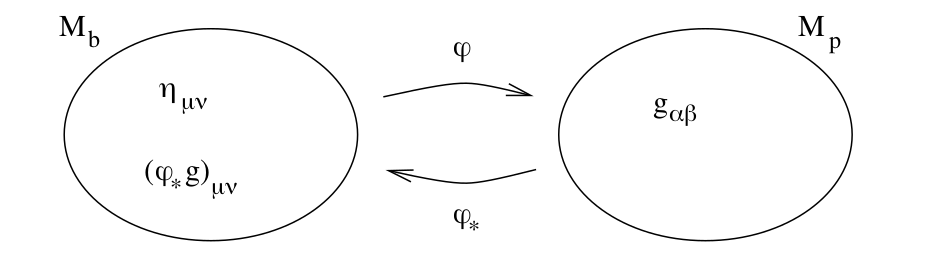
\includegraphics[width=0.7\linewidth]{gfx/GaugeInvarianceGR}
	\caption{}
	\label{fig:gaugeinvariancegr}
\end{figure}





\begin{statements}
	\textbf{In this language, the issue of gauge invariance is simply the fact that there are a large
	number of permissible diffeomorphisms between $M_b$ and $M_p$ (where “permissible” means that the perturbation is small).}
\end{statements}
Consider a vector field $\xi^μ (x)$ on the background spacetime.
This vector field generates a one-parameter family of diffeomorphisms $ψ_\epsilon : M_b → M_b$ . For
$\epsilon$ sufficiently small, if $\phi$ is a diffeomorphism for which the perturbation defined by $	h_{\mu \nu} = (\phi^* g)_{\mu \nu} -\eta_{\mu \nu}.$ is
small than so will $(\phi \circ ψ_\epsilon )$ be, although the perturbation will have a different value.
\begin{figure}[h!]
	\centering
	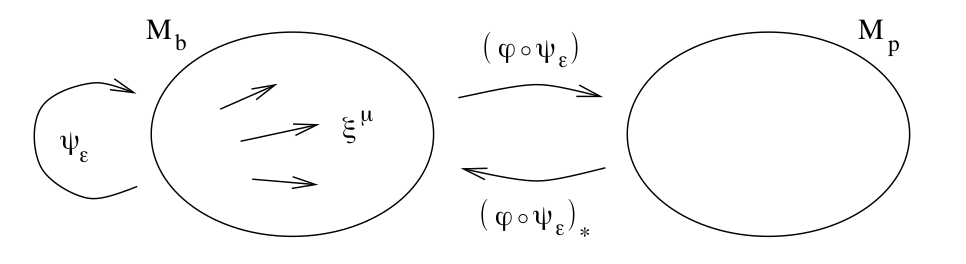
\includegraphics[width=0.7\linewidth]{gfx/GaugeInvarianceGr2}
	\caption{}
	\label{fig:gaugeinvariancegr2}
\end{figure}

Specifically, we can define a family of perturbations parameterized by $\epsilon$:
\begin{align*}
	h^{(\epsilon )}_{\mu \nu} &= [(\phi \circ ψ_\epsilon )_* g]_{ μν} − η_{μν}\\
	&= [ψ_{\epsilon_*} (φ_* g)]_{ μν} − η_{ μν}.
\end{align*}
The second equality is based on the fact that the pullback under a composition is given by
the composition of the pullbacks in the opposite order, which follows from the fact that the
pullback itself moves things in the opposite direction from the original map. Plugging in the
perturbation, we find
\begin{align}
	h^{(\epsilon)}_{\mu \nu} &= ψ_{\epsilon_*} (h + η)_{μν} − η_{μν} \\
	&= \psi_{\epsilon_*}(h_{\mu\nu}) + \psi_{\epsilon_*} (\eta_{\mu \nu}) - \eta_{\mu \nu} 
\end{align}
(since the pullback of the sum of two tensors is the sum of the pullbacks). Now we use our
assumption that $\epsilon$ is small; in this case $\psi_{\epsilon_*}(h_{μν} )$ will be equal to $h_{μν}$ to lowest order, while
the other two terms give us a Lie derivative:
\begin{align}
	\label{eq:GaugefreedomGR}
	h^{(\epsilon)}_{\mu \nu} &= \psi_{\epsilon_*}(h_{\mu \nu}) + \epsilon \left[ \frac{\psi_{\epsilon_*}(\eta_{\mu \nu}) - \eta_{\mu \nu}}{\epsilon}\right]\\
	&= h\munu +\epsilon \mL_\xi \eta_{\mu \nu} \\
	&= h\munu + 2 \epsilon \partial_{(\mu}\xi_{\nu)}.
\end{align}
The last equality follows from our previous computation of the Lie derivative of the metric \ref{eq:liederivMetric}, plus the fact that covariant derivatives are simply partial derivatives to lowest order.\\
\textbf{The infinitesimal diffeomorphisms $\psi_{\epsilon}$ provide a different representation of the same physical situation, while maintaining our requirement that the perturbation be small. Therefore,
the result \ref{eq:GaugefreedomGR} tells us what kind of metric perturbations denote physically equivalent
spacetimes — those related to each other by $2\epsilon ∂_{ (μ} ξ_{ ν)}$ , for some vector $ξ^μ$ }. The invariance of our theory under such transformations is analogous to traditional gauge invariance of electromagnetism under $A_μ → A_μ + ∂_μ λ$. (The analogy is different from the previous analogy
we drew with electromagnetism, relating local Lorentz transformations in the orthonormal-
frame formalism to changes of basis in an internal vector bundle.) In electromagnetism the
invariance comes about because the field strength $F_{μν} = ∂_μ A_ν − ∂_ν A_μ$ is left unchanged
by gauge transformations; similarly, \textbf{we find that the transformation \ref{eq:GaugefreedomGR} changes the linearised Riemann tensor by $\delta R_{\mu \nu \rho \sigma}=0$, i.e. the physical situations are the same},  as was computed in exercises. Our abstract derivation of the appropriate gauge transformation for the metric perturbation is verified by the fact that it leaves the curvature (and hence the physical spacetime)
unchanged.

\item Gauge invariance can also be understood from the slightly more lowbrow but considerably
more direct route of infinitesimal coordinate transformations. Our diffeomorphism $ψ_\epsilon$ can
be thought of as changing coordinates from $x^μ$ to $x^μ − \epsilon ξ^μ$ . (The minus sign, which is
unconventional, comes from the fact that the “new” metric is pulled back from a small
distance forward along the integral curves, which is equivalent to replacing the coordinates
by those a small distance backward along the curves.) Following through the usual rules for
transforming tensors under coordinate transformations, you can derive precisely \ref{eq:GaugefreedomGR} —
although you have to cheat somewhat by equating components of tensors in two different
coordinate systems, c.f. Weinberg.
\end{enumerate}
When faced with a system that is invariant under some kind of gauge transformations,
our first instinct is to fix a gauge. We have already discussed the harmonic coordinate
system, and will return to it now in the context of the weak field limit.
\\
\\
INCORPORATE INTO THE ABOVE:\\
What is gauge invariance ?\\
The equations of physics are invariant when we make  coordinate displacements any constant amount $a^\mu$ :
\begin{equation}
x^{\mu^\prime} = x^\mu +a^\mu.
\end{equation}
To make it formally more like the phase (in qm. $\psi^\prime = e^{ia} \psi$) and isospin (Yang-Mills vector meson theory: $\psi^\prime = e^{i \vec{\tau}\cdot \vec{a}} \psi$, the proposal of Yang and Mills is that a field should be aded to the Lagrangian, in such a way that a \emph{space-dependent} phase change $\vec{a}\rightarrow \vec{X}$ makes no difference in the equations) transformations, one might use the momentum representation so that the translation operator is
\begin{equation}
\exp(i p_\mu a^\mu).
\end{equation}
On the other hand, it is possible to investigate how we might make the equations of physics invariant when we allow space dependent \emph{variable} displacements $a^\mu \rightarrow \zeta^\mu$. The search will be for a more complete Lagrangian, the new terms that are needed are precisely those of a gravity field. Thus, gravity is that field which corresponds to a gauge invariance with respect to displacement transformations. MORE LATER






\subsection{Linearised theory of gravity}
\marginpar{Excellently satisfied in the solar system or galaxy cluster with high $\Phi \Rightarrow$ Pull indices up and down with $\eta_{\mu \nu}$ and not $g_{\mu\nu}$ to remain leading order $\mathcal{O}(h^2)$.}
Study solutions for the field equations in the case of an almost Minkowskian metric, i.e with small perturbation
\begin{equation}
g_{\mu \nu} = \eta_{\mu \nu} + h_{\mu \nu}, 
\end{equation}
with $|h_{\mu \nu}|\ll 1$, this is a coordinate dependent condition, can be violated in other system.
Note that the perturbations
can be split up into \emph{scalar} perturbations $( h_{ 00} , h_{ii} )$, \emph{vector} perturbations ( $h_{0i}$ ) and \emph{tensor} perturbations $h_{i j}$ . At
first order they correspond to gravitational potentials, gravitomagnetic effects and waves respectively.\\
 \\
We can think of
the linearised version of general relativity (where effects of higher than first order in $h_{μν}$
are neglected) as describing a theory of a symmetric tensor field $h_{μν}$ propagating on a flat
background spacetime. This theory is Lorentz invariant in the sense of special relativity;
under a Lorentz transformation $x^{μ^\prime} = Λ^{\mu^\prime}_μ x^μ$ , the flat metric $η_{μν}$ is invariant, while the
perturbation transforms as a symmetric tensor does under Lorentz trafo
(Note that we could have considered small perturbations about some other background
spacetime besides Minkowski space. In that case the metric would have been written $g_{μν} =g^{(0)}_{μν}+ h_{μν}$ , and we would have derived a theory of a symmetric tensor propagating on the
curved space with metric $g^{(0)}_{ μν}$. Such an approach is necessary, for example, in cosmology.)
\\
\\
The weak metric perturbation $h_{\mu \nu}$ admits the gauge transformation
\begin{equation}
	h_{\mu \nu} \rightarrow h_{\mu \nu} + \partial_{\mu} \xi_{\nu} + \partial_{\nu} \xi_{\mu},
\end{equation}
where $\xi=vt$. This is the \emph{gauge class}. One can change $h_{\mu \nu}$ in this way without violating physical laws, this is the \emph{gauge freedom} as described above for the lecture definition of diffeomorphism invariance. Note
that the linearised (in $h$) Ricci tensor is
\begin{equation}
	R\munu =\half η^{αβ}\left[ ∂_μ ∂_β h_{αν} + ∂_α ∂_ν h_{μβ} − ∂_α ∂_β h_{μν} − ∂_μ ∂_ν h_{αβ} \right] 
\end{equation}
is invariant under this gauge transformation, which exemplifies that the gauge transformation relates two situations which are physically \emph{equivalent}.
\begin{mybox}{Gauge theories}
	A gauge theory represents each physically distinct configuration of the system as an equivalence class of detailed local field configurations. Any two detailed configuration in the same equivalence class are related by a gauge transformation, as e.g. above.
\end{mybox}
\begin{mybox}{Hilbert gauge}
The harmonic gauge $\nabla^\nu \nabla_\nu x^\mu=g^{\rho \lambda} \Gamma^\mu_{\rho \lambda}=0$ in the weak field limit is equivalent to
\begin{equation}
\label{eq:Hilbertgauge}
	\half \eta^{\mu \nu} \eta^{\lambda \rho} \left[\partial_{(\mu} h_{\nu \lambda} + \partial_{\nu} h_{\lambda \mu} - \partial_{\lambda} h\munu\right]=\underbrace{∂_μ h^\mu_λ −\half  ∂_λ h}_{\partial\mu \gamma^\mu_{\,\, \lambda}} = 0 .
\end{equation}
This condition is also known as \emph{Lorentz gauge (or Einstein gauge or Hilbert gauge or de Don-
der gauge or Fock gauge)}. As before, we still have some gauge freedom remaining, since we
can change our coordinates by (infinitesimal) harmonic functions.
\end{mybox}
Substituting 
\begin{equation}
	\gamma_{\mu \nu} = h_{\mu \nu} - \frac{1}{2} \eta_{\mu \nu} \underbrace{h^a_a}_{:= h}
\end{equation}
and enforcing the \emph{Hilbert gauge condition}
\begin{equation}
	\partial_{\nu} \gamma^{\mu \nu} = 0,
\end{equation}
in order to have gauge invariance made physical $\Leftrightarrow$ coping with redundant degrees of freedom due to the gauge invariance, to find the linearised field equations as
\begin{equation}
\label{eq:eomlinearisedperturbationsGR}
	\square \gamma^{\mu \nu} = -\frac{16 \pi \mathcal{G}}{c^4} T^{\mu \nu}.
\end{equation}
The vacuum equations $R_{μν} = 0$ take on the elegant form
\begin{equation}
\label{eq:eomvacuumlinearisedpeturbationGR}
	\square \gamma_{\mu \nu} =0
\end{equation}
which is simply the conventional relativistic wave equation. Together, \ref{eq:eomvacuumlinearisedpeturbationGR} and \ref{eq:Hilbertgauge}
determine the evolution of a disturbance in the gravitational field in vacuum in the harmonic
gauge.\\
We can use the QED solution (its retarded Green's function) here since both theories are mediated by massless bosons (otherwise Yukawa cut-off $\frac{1}{|x-x'|} \mapsto \frac{1}{|x-x'|} e^{- |x-x'|\lambda}$). \\
Formally being identical to the Maxwell equations, these equations can therefore be solved using the retarded Green's function of Maxwell electrodynamics. Thus, similar to electrodynamics, the metric perturbation consists of the field generated by the source plus wave-like vacuum solution propagating \emph{at} the speed of light, i.e. \emph{gravitational waves} with $v=c$.

\subsection{Nearly Newtonian gravity}
\todo{Go through chapter 10 gravitational radiation by Weinberg and incorporate into this sparse treatment of the topic.}
Now one can insert all kinds of specific sources into $T_{\mu \nu}$ to determine the metric, since $T_{\mu \nu}$ determines $\gamma_{\mu \nu}$.\\
In the non-relativistic case $T_{00} \gg |T_{0j}| \; \& \; T_{00} \gg |T_{ij}|$, we recover the \emph{Newtonian approximation} of the metric.
From \ref{eq:eomlinearisedperturbationsGR} and our previous exploration of the Newtonian limit, it is straightforward to
derive the weak-field metric for a stationary spherical source such as a planet or star. Recall
that previously we found that Einstein’s equations predicted that $h_{00}$ obeyed the Poisson
equation in the weak-field limit, which implied
$h_{00} = −2Φ$, where $Φ$ is the conventional Newtonian potential, $Φ = −GM/r$. Let us now assume that
the energy-momentum tensor of our source is dominated by its rest energy density $ρ = T_{00}$ .
(Such an assumption is not generally necessary in the weak-field limit, but will certainly
hold for a planet or star, which is what we would like to consider for the moment.) Then
the other components of $T\munu$ will be much smaller than $T_{00}$ , and from \ref{eq:eomlinearisedperturbationsGR} the same must
hold for $\gamma_{\mu \nu}$ . If $\gamma_{00}$ is much larger than $\gamma_{ij}$ , we will have
\begin{equation}
	h = -\gamma = -\eta^{\mu \nu} \gamma_{\mu \nu} = \gamma_{00},
\end{equation}
and then we immediately find
\begin{equation}
\gamma_{00} = 2 h_{00} = - 4\Phi.
\end{equation}
The other components of $\gamma_{μν}$ are negligible, from which we can derive
\begin{equation}
	h_{i0} = \gamma_{i0} - \half \eta_{0i}\gamma =0
\end{equation}
and 
\begin{equation}
	h_{ ij} = \gamma_{ij} − \half \eta_{ ij} \gamma = −2Φ δ_{ij}.
\end{equation}
The metric for a star or planet in the weak-field limit is therefore
\begin{equation}
	\md s^2 = -(1+2 \Phi) \md t^2 + (1 -2 \Phi) \md \vec{x}^2.
\end{equation}




\begin{mybox}{Newtonian limit}
	In the Newtonian limit (non-relativistic limit +weak gravitational field+instantaneous propagation of perturbations), the weakly perturbed metric of a mass $M$ has the line element
	\begin{align}
		\md s^2 &= - \left(1+ \frac{2 \Phi}{c^2}\right) c^2 \md t^2 + \left(1-\frac{2 \Phi}{c^2}\right) \md \vec{x}^2,\\
		\Leftrightarrow \md s^2 &=-\left(1 - \frac{2 \mathcal{G}M}{r c^2}\right) c^2 \md t^2 + \left(1+\frac{2 \mathcal{G}M}{r c^2}\right) \md \vec{x}^2\\
		\Rightarrow (g_{\mu \nu}) &= (\eta_{\mu \nu}) - \frac{2 \Phi}{c^2} \mathcal{I}_{4\times 4}.
	\end{align}
\end{mybox}

Thus, the full theory has space-time curvature \emph{and} not only spatial curvature.\\
Note: \\
Although we have now imposed the harmonic gauge condition, there is still some coordinate freedom left. Remember that any coordinate transformation of the form
$x^μ → x^μ + ζ^μ$ will leave the harmonic coordinate condition $\nabla^\alpha \nabla_\alpha x^μ = 0$ satisfied as long as we have $\nabla^\alpha \nabla_\alpha ζ^μ = 0$.
Conclusions:
\begin{enumerate}
	\item Light follows null geodesics $\md s^2=0 \Rightarrow$ velocity of light in gravitational field is less than $c$:
	\begin{equation}
	\frac{\md \vec{x}^2}{\md t^2} = c^2 \frac{\left(1+\frac{2 \Phi}{c^2}\right)}{\left(1-\frac{2 \Phi}{c^2}\right)} =: (c')^2 \; \Rightarrow \; c' = \frac{c}{n}, n \approxeq 1-\frac{2 \Phi}{c^2}.
	\end{equation}
	\begin{mybox}{Gravitational Lensing}
		A weak gravitational field with Newtonian gravitational potential $\Phi$ has the effective index of refraction
		\begin{equation}
		n = 1- \frac{2 \Phi}{c^2} \geq 1, 
		\end{equation}
		$\Rightarrow$ optically denser medium than vacuum\\
		$\Rightarrow$ Light deflection, light rays are bent in a gravitational field.
	\end{mybox}
	\item \emph{Clocks go slower in a gravitational field}:\\
	\marginpar{The gravitational potentials are negative, so that clock should run more slowly as they come nearer to a massive object such as a star.}
	Compared to light propagation in vacuum, there is thus a \emph{time delay}
	\begin{equation}
		\Delta(\md t) = \md t-\frac{\md l}{c} = - \frac{2 \Phi}{c^3} \md l,
	\end{equation}
	with $\md t=\frac{\md l}{c'}= n \frac{\md l}{c}$ the light travel time along an infinitesimal path length $\md l$ in a gravitational field (hence $c'$).\\
	With respect to whom do clocks go slower ?\\
	Suppose two clocks are at rest. The clock that is under the influence of a stronger gravitational
	field (i.e. it is closer to a massive object) ticks slower than the other clock experiencing a weaker
	gravitational field (i.e. it is farther away from the massive object).
\end{enumerate}

Introducing outer source $T_{\mu \nu}$ leads to the \emph{gravitomagnetic field}. Only approximate $T_{ij}=0$ (no stresses) and define $A_{\mu} = \gamma_{0 \mu} /4$ to find
\begin{equation}
	\square A_{\mu} = - \frac{4 \pi}{c^2} \underbrace{j_{\mu}}_{=\frac{\mathcal{G}T_{0 \mu}}{c^2}}.
\end{equation}
This similarity to electrodynamics leads to the introduction of "electric" and "magnetic" components of the gravitational field.
\begin{statements}
	Matter currents create a magnetic gravitational potential $A_{\mu}$ ("gravitomagnetic potential") similar to the em. vector potential $A_{\nu}$.
\end{statements}
$\Rightarrow T_{\mu \nu}$ yields the metric, which in turn yields the e.o.m. via the variational principle !.\\
\marginpar{This treatment is only an analogy! If you have to take matter currents $T_{0j}$ into account in gavitational field, then you get similar behaviour as in ED. Before we only used matter densities.}
$\Rightarrow$ One recovers e.o.m. which exhibit a "magnetic" Lorentz force term and a gravitational term. Its effect on a spinning test particle is the \emph{gravito-magnetic force} $\vec{f} = c^2\vec{\nabla} A_0 + 4 c \vec{v} \times \vec{B}$, with $\vec{B}:= \vec{\nabla} \times \vec{A}$, lets the test particles' angular momentum experience a torque:
\begin{mybox}{Lense-Thirring effect or space time frame drag}
	A spinning body in a gravitomagnetic field will experience spin precession with the angular frequency \begin{equation}
		\vec{\omega} = -2 c \vec{B} = - 2 c\vec{\nabla }\times \vec{A},
	\end{equation}
	which is called the Lense-Thirring effect.\\
	$\Leftrightarrow$ A rotating body drag the gravitational field in its vicinity around.\\
	It predicts that the rotation of a massive object would distort the spacetime metric, making the orbit of a nearby test particle precess. This does not happen in Newtonian mechanics for which the gravitational field of a body depends only on its mass, not on its rotation. The Lense–Thirring effect is very small—about one part in a few trillion. To detect it, it is necessary to examine a very massive object, or build an instrument that is very sensitive.
\end{mybox}

Frame-dragging is an effect on spacetime that is due to non-static stationary distributions of mass–energy. A stationary field is one that is in a steady state, but the masses causing that field may be non-static, rotating for instance. More generally, the subject of effects caused by mass–energy currents is known as gravitomagnetism, in analogy with classical electromagnetism. The Lense-Thirring effect is one spacetime frame dragging effect, the rotational frame-dragging.
\\
The possible frame-dragging effects are:\\
\begin{enumerate}
	\item \emph{Rotational frame-dragging (the Lense–Thirring effect)} appears in the general principle of relativity and similar theories in the vicinity of rotating massive objects. 
	Under the Lense–Thirring effect, the frame of reference in which a clock ticks the fastest is one which is revolving around the object as viewed by a distant observer. This also means that light travelling in the direction of rotation of the object will move past the massive object faster than light moving against the rotation, as seen by a distant observer. It is now the best known frame-dragging effect, partly thanks to the Gravity Probe B experiment. Qualitatively, frame-dragging can be viewed as the gravitational analogue of electromagnetic induction.\\
	\\	
	Also, an inner region is dragged more than an outer region. This produces interesting locally rotating frames. For example, imagine that a north-south–oriented ice skater, in orbit over the equator of a black hole and rotationally at rest with respect to the stars, extends her arms. The arm extended toward the black hole will be "torqued" spinward due to gravitomagnetic induction ("torqued" is in quotes because gravitational effects are not considered "forces" under GR). Likewise the arm extended away from the black hole will be torqued anti-spinward. She will therefore be rotationally sped up, in a counter-rotating sense to the black hole. This is the opposite of what happens in everyday experience. There exists a particular rotation rate that, should she be initially rotating at that rate when she extends her arms, inertial effects and frame-dragging effects will balance and her rate of rotation will not change. Due to the equivalence principle, gravitational effects are locally indistinguishable from inertial effects, so this rotation rate, at which when she extends her arms nothing happens, is her local reference for non-rotation. This frame is rotating with respect to the fixed stars and counter-rotating with respect to the black hole. This effect is analogous to the hyperfine structure in atomic spectra due to nuclear spin. A useful metaphor is a planetary gear system with the black hole being the sun gear, the ice skater being a planetary gear and the outside universe being the ring gear. See Mach's principle.\\
	\\
	Another interesting consequence is that, for an object constrained in an equatorial orbit, but not in freefall, it weighs more if orbiting anti-spinward, and less if orbiting spinward. For example, in a suspended equatorial bowling alley, a bowling ball rolled anti-spinward would weigh more than the same ball rolled in a spinward direction. Note, frame dragging will neither accelerate nor slow down the bowling ball in either direction. It is not a "viscosity".\todo{What does that mean, how is the equivalence and not feeling gravity compatible with this ? EP says that gravity is not distinct able from an acceleration, but the objects weighs more moving against or less if moving with rotation of the BH ? } Similarly, a stationary plumb-bob suspended over the rotating object will not list. It will hang vertically. If it starts to fall, induction will push it in the spinward direction.
	
	\item \emph{Linear frame dragging} is the similarly inevitable result of the general principle of relativity, applied to linear momentum. Although it arguably has equal theoretical legitimacy to the "rotational" effect, the difficulty of obtaining an experimental verification of the effect means that it receives much less discussion and is often omitted from articles on frame-dragging (but see Einstein, 1921).
	
	\item \emph{Static mass increase} is a third effect noted by Einstein in the same paper. The effect is an increase in inertia of a body when other masses are placed nearby. While not strictly a frame dragging effect (the term frame dragging is not used by Einstein), it is demonstrated by Einstein that it derives from the same equation of general relativity. It is also a tiny effect that is difficult to confirm experimentally.
	
	
\end{enumerate}


















\section{Gravitational Waves - The propagation of the metric perturbations}
\todo{This is treated in way more detail in Caroll, c.f. page 148.}
Describing gravitational perturbations as superposition of plane waves
\begin{equation}
	\gamma_{\mu \nu} = \mathrm{Re}\{ \epsilon_{\mu \nu} e^{i \langle k,x\rangle} \},
\end{equation}
\marginpar{For gauge trafo $h_{\mu \nu} \rightarrow h_{\mu \nu} + \partial_{\mu} \xi_{\nu}+\partial_{\nu} \xi_{\mu}$ with
$2 \partial_{\mu}\xi^{\mu}=0, \partial_{\alpha}\partial^{\alpha} \xi^{\mu} =0$ in Hilbert gauge, one has
$\gamma_{\mu \nu}=h_{\mu \nu}$.}
with amplitudes given by the so-called polarisation tensor $\epsilon_{\mu \nu}$, one finds in Hilbert gauge:
\begin{mybox}{Gauge-invariant polarisation states}
	As for electromagnetic waves, there are only two gauge-invariant, linearly independent polarisation states for gravitational waves.\\
	$h=\pm 2 \Rightarrow$ the two polarisation states correspond to left and right-handed circular polarisation.
\end{mybox}
In the limit of far-away source, small velocities and overall rest-mass dominating, one finds 
\marginpar{Em waves are created by time-dependent dipole instead.}
\begin{mybox}{Source of gravitational waves I}
	Wave-like metric perturbations in varuum are created by the second time-derivative of a matter distribution with density $\rho$,
	\begin{align}
		\gamma^{jk} (t,\vec{x}) &= -\frac{2\mathcal{G}}{r c^4} \partial^2_t \int \rho \left(t-\frac{r}{c}, \vec{x}\right) x^{'j} x^{'k} \md^3 x', \\
		\gamma_{jk}(t,\vec{x}) &= -\frac{2 \mathcal{G}}{3 r c^4} \left[\partial^2_t Q_{jk} \left(t-\frac{r}{c}, \vec{x}\right) \right. \nonumber \\
		&\left. + \delta_{jk} \partial^2_t \int r^{'2} \rho \left(t-\frac{r}{c}, \vec{x}'\right) \md^3 x'\right],\\
		Q^{jk} &= \int \left(3 x^j x^k -r^2 \delta^{jk} \right) \rho(\vec{x}) \md^3x,
	\end{align}
where $Q^{jk}$ is the source's quadrupole tensor
\end{mybox}
\begin{mybox}{Source of gravitational waves II}
	In order to generate gravitational waves, a mass distribution needs to have a quadrupole moment with non-vanishing second time derivative.
\end{mybox}
The physical reason is the following. The mass monopole represents the total mass-energy in a system, which is conserved. Thus, it cannot lead to radiation. Similarly, the mass dipole corresponds to the centre of mass of a system and its first derivative represents momentum, which is also a conserved quantity so that the mass dipole cannot emit radiation either. The second derivative of the mass quadrupole, however, does not vanish so that the quadrupole is the lowest-order contribution to gravitational radiation. The gravitational wave produced by an isolated nonrelativistic object is therefore proportional to the second derivative of the quadrupole moment of the energy density at the point where the past light cone of the observer intersects the source. In contrast, the leading
contribution to electromagnetic radiation comes from the changing dipole moment of the
charge density. The difference can be traced back to the universal nature of gravitation. A
changing dipole moment corresponds to motion of the center of density — charge density in
the case of electromagnetism, energy density in the case of gravitation. While there is nothing to stop the center of charge of an object from oscillating, oscillation of the center of mass
of an isolated system violates conservation of momentum. (You can shake a body up and
down, but you and the earth shake ever so slightly in the opposite direction to compensate.)
The quadrupole moment, which measures the shape of the system, is generally smaller than
the dipole moment, and for this reason (as well as the weak coupling of matter to gravity)
gravitational radiation is typically much weaker than electromagnetic radiation.
\\
\\
Einstein's quadrupole formula describes the gravitational-wave luminosity
\begin{equation}
	L_{\mathrm{GW}} = \frac{\mathcal{G}}{5 c^5} \langle \tr(\dddot{Q})^2\rangle.
\end{equation}




























\newpage
\section{The Schwarzschild solution}
\subsection{Stationary and static space-times}
\emph{Stationary Spacetimes} $(M,g)$ are defined to be spacetimes which have a global time-like Killing vector field $K$. This means that observers moving along the integral curves of $K$ do not notice any change. This definition implies that we can introduce coordinates in which the components $g_{\mu \nu}$ of the metric do not depend on time. In these so-called \emph{adapted coordinates} with $g_{\mu \nu}(t)=g_{\mu \nu}$, one transports every point on the manifold along the integral-curve of $K = (\partial_0,0,0)$, i.e. along global time coordinates with ($\mathcal{L}_K g)_{\mu \nu} = 0 = \partial_0 g_{\mu \nu}$.\\
\marginpar{$K$ time-like $\Rightarrow \Sigma$ space-like since $K\perp\Sigma$ at $t=t_0$.}\\
In a stationary space-time with time-like Killing vector field $K$, the \emph{Frobenius condition}
\begin{equation}
	\omega \wedge \md \omega =0
\end{equation}
for the one-form $\omega=K^{\flat}$ is equivalent to the condition
\begin{equation}
	g_{0i}=0, \quad  \Rightarrow K\perp \Sigma \,\mathrm{for\, which} \,t=\mathrm{constant},
\end{equation}
which implies that there is no rotation in spacetime, in adapted coordinates ($\Leftrightarrow \md s^2 = \md s^2_{\Sigma} - \md t^2$ decouples spatial and time contributions).\\
Such space-times are called \emph{static}.\\
$\Rightarrow$ In static spacetimes, the metric can thus be written in the form
\begin{equation}
	g = g_{00}(\vec{x}) c^2 \md t^2 + g_{ij}(\vec{x}) \md x^i \md x^j.
\end{equation}
Saying that $K=\partial_t$ is irrotational means that the vorticity tensor of the corresponding timelike congruence vanishes, thus the Killing vector field is the hypersurface orthogonal $K\perp\Sigma$. One immediate consequence is that the constant time coordinate surfaces $t=t_0$ form a family of (isometric) spatial hyperslices.
\begin{figure}
	\centering
	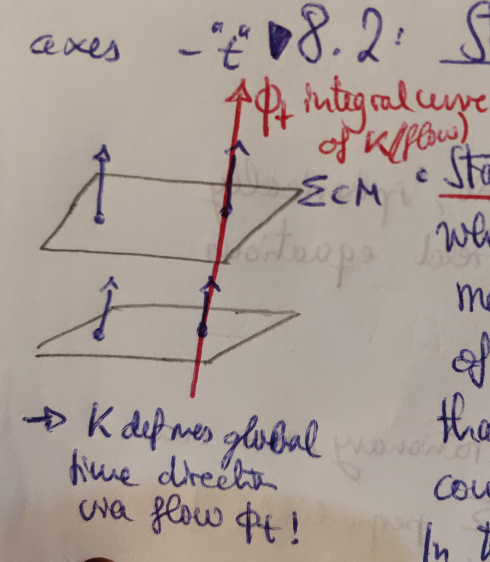
\includegraphics[width=0.7\linewidth]{gfx/staticspacetime}
	\caption{\itshape Foliation of the static spacetime along the fiducial time direction given by global Killing vector field.}
	\label{fig:staticspacetime}
\end{figure}
Roughly speaking, a static metric is one in which nothing is moving,
while a stationary metric allows things to move but only in a symmetric way. For example,
the static spherically symmetric metric (Schwarzschild) will describe non-rotating stars or black holes,
while rotating systems (which keep rotating in the same way at all times) will be described
by stationary metrics.
 \subsection{The Schwarzschild solution}

 The Schwarzschild solution is a static, spherically symmetric solution of Einstein's field equations for vacuum space-time. It describes the gravitational field \emph{outside} a spherical mass, on the assumption that $Q(\mathrm{mass})=\vec{L}(\mathrm{mass})=0=\Lambda$. It works well for slowly rotating astronomical objects (stars, planets). Birkhoff’s theorem states that the
 Schwarzschild solution is the unique spherically symmetric solution to Einstein’s equations
 in vacuum.\\ The Schwarzschild chart is adapted to the spheres $S^2$ nested in Schwarzschild spacetime.\\
 \\
 As the space-time is (globally) stationary, we can introduce spatial hypersurfaces $\Sigma$ perpendicular to the time-like Killing vector field, which in adapted coordinates is $K=\partial_0$. The manifold $(M,g)$ can thus be foliated as $M \cong \mR \times \Sigma$.\\
 \\
 The spatial hypersurfaces $ \Sigma$ are expected to be spherically symmetric, i.e. $SO(3)$ must be an isometry group of the metric $\mathcal{h}$ of the spatial sections 
$h$. The orbits of $SO(3)$ are two-dimensional, space-like surfaces in $\Sigma$. Thus, $SO(3)$ foliates the spacetime $(\Sigma, h)$ into invariant two-spheres.\\
Let the surfaces of these two-spheres be $A$, then we \emph{define} a radial coordinate for the Schwarzschild metric requiring $A=4 \pi r^2$ as in Euclidean geometry. The spherical symmetry further implies that we can introduce spherical polar coordinates $(\vartheta,\varphi)$ on one particular orbit of $SO(3)$ which can then be transported along geodesic lines perpendicular to the orbits.\\
$\Rightarrow$ The spatial sections $\Sigma$ are now foliated according to 
\begin{equation}
	\Sigma = I \times S^2, \; I\subset \mR^+, \quad \mathrm{for} \;r\in I, (\vartheta, \varphi) \in S^2.
\end{equation}
\marginpar{static implies $a(r,t)=a(r)$, such that space-time cannot expand or shrink with time.}
\begin{mybox}{Metric for static, spherically space-times}
	In the Schwarzschild coordinates $(t,r,\vartheta,\varphi)$, the metric of a static, spherically-symmetric space-time has the form
	\begin{equation}
		g = - e^{2 a(r)} c^2 \md t^2 + e^{2 b(r)} \md r^2 + r^2 \md \Omega^2.
	\end{equation}
	The functions $a(r), b(r)$ are constrained by the requirement that the metric should asymptotically turn flat, which means $a(r),b(r) \stackrel{r \rightarrow \infty}{\longrightarrow} 0$, They must be determined by inserting the metric into the vacuum field equations, $G=0$.
\end{mybox}
Introduce tetrad $\{e_i\}$ or alternatively dual-tetrad $\{\theta^i\}$:
\begin{equation}
	\underbrace{\theta^0 = e^a c \md t }_{\Leftrightarrow \theta^0=(e^a,0,0,0)}, \quad \theta^1 = e^b \md r, \quad \theta^2=r \md \vartheta, \quad \theta^3=r \sin\vartheta \md \varphi.
\end{equation}
In terms of this dual-tetrad, the metric attains the simple diagonal, Minkowskian form
\begin{equation}
	g =g_{\mu \nu} \theta^{\mu} \otimes \theta^{\nu}, \qquad g_{\mu \nu} = \mathrm{diag}(-1,1,1,1), \Rightarrow \md g=0.
\end{equation}
For a torsion-free connection, one can then determine the connection form via Cartan $I$ \ref{eq:cartanStructure}. Via Cartan $II$, the curvature forms are found.
\subsection{Solution of the field equations}
With the curvature forms in the given tetrad at hand, one finds the Ricci tensor and thus the Einstein tensor via
\begin{equation}
	R_{\mu \nu} = \bar{R}^{\lambda}_{\mu \lambda \nu} = \Omega^{\lambda}_{\mu}(e_{\lambda}, e_{\nu}).
\end{equation}
\textbf{All off-diagonal components of $G_{\mu \nu}$ vanish identically, which reflects the spherical symmetry of the considered system}.\\
\begin{mybox}{Einstein tensor for a static, spherically-symmetric metric}
	The Einstein tensor of a static, spherically-symmetric metric has the
	components
	\begin{align}
		G_{00} &=\frac{1}{r^2} - E\left(\frac{1}{r^2} - \frac{2 b^\prime}{r}\right), \quad E:= \exp(-2b(r))\\
		G_{11} &=- \frac{1}{r^2}+ E\left(\frac{1}{r^2}+ \frac{2 a^\prime}{r}\right)\\
		G_{22} &= G_{33}.
	\end{align}
All off-diagonal components of $G\munu$ vanish identically.
\end{mybox}
$G_{00}=G_{11}=G_{22}=0$, and thus also $G_{00}+G_{11}=0$ etc, are now differential equations in $a$ and $b$, which can be solved via our boundary condition of asymptotic flatness.
\begin{mybox}{Schwarzschild line element}
	This yields the Schwarzschild solution for the metric,
	\begin{equation}
	\label{eq:Schwarzschildmetric}
		\md s^2 = -\left(1-\frac{2m}{r}\right) c^2 \md t^2 + \frac{\md r^2}{1-\frac{2m}{r}} + r^2 \md \Omega^2.
	\end{equation}
\end{mybox}
Note that $M$ is precisely equal to the total energy of the sun \emph{and its gravitational field} here. The total energy of matter and gravitation here is
\begin{equation}
	P^0 = M,
\end{equation}
where one furthermore finds that the total angular momentum is the expected value zero.

\begin{figure}
	\centering
	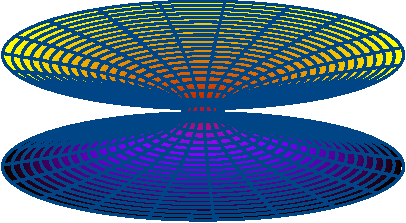
\includegraphics[width=0.7\linewidth]{gfx/schwarzschildMetric}
	\caption{\itshape Schwarzschild spacetime with a physical singularity at $r=0$.}
	\label{fig:schwarzschildmetric}
\end{figure}
In the weak field limit, we have to recover the Newtonian limit $g_{00} \mapsto - (1+\frac{2 \Phi}{c^2})$. We describe a point mass $M$ at the origin with this metric and have $\Phi=-\frac{\mathcal{G}M}{r}$ for $r\gg0$.
\begin{equation}
	\stackrel{\md s^2}{\Rightarrow} \frac{2m}{r} \stackrel{!}{=} \frac{2 \mathcal{G}M}{r c^2} \; \Leftrightarrow\; m:= \frac{\mathcal{G}M}{c^2} = \frac{R_s}{2}.
\end{equation}
The Schwarzschild metric has a coordinate singularity at $r=2m$ or
\begin{equation}
	r=R_s= \frac{2 \mathcal{G}M}{c^2},
\end{equation}
the so-called \emph{Schwarzschild radius}.

\subsubsection{Equivalent forms of the metric}
\begin{enumerate}
	\item We can equivalently express the Schwarzschild metric \ref{eq:Schwarzschildmetric} in the \emph{isotropic form}, by introducing a new radius variable
	\begin{equation}
	\rho \equiv \half \left[r-m+\sqrt{r^2- 2mr}\right] \quad \Leftrightarrow\quad r = \rho (1 + \frac{m}{2 \rho})^2,
	\end{equation}
	which yields the line element
	\begin{equation}
		\md \tau^2 = \left(\frac{1 - \frac{m}{2 \rho}}{1+\frac{m}{2 \rho}}\right)^2 c^2 \md t^2 - \left(1+\frac{m}{2 \rho}\right)^4 \left(\md \rho^2 + \rho^2 \md \theta^2 + \rho^2 \sin^2 \theta \md \varphi^2\right).
	\end{equation}
	\item We can also construct \emph{harmonic coordinates}
	\begin{equation}
		X_1 = R\sin\theta \cos \varphi , \quad X_2 = R\sin\theta\sin\varphi,\quad X_3=R\cos\theta,\quad t
	\end{equation}
	by using for $R$ a solution of a TODO maybe.
\end{enumerate}

\subsection{Birkhoff's theorem}
\label{subsubsec:BirkhoffTheorem}
\begin{mybox}{Birkhoff's theorem}
	In general relativity, Birkhoff's theorem states that any spherically symmetric solution of the vacuum field equations must be static and asymptotically flat. This means that the exterior solution (i.e. the spacetime outside of a spherical, nonrotating, gravitating body) must be given by the Schwarzschild metric.\\
	Thus, a spherically symmetric solution of Einstein's vacuum equations is necessarily static for $r>2m$.\\
	 $\Leftrightarrow$ the Schwarzschild metric is the unique solution to the Einstein equations in vacuum with a spherically symmetric matter distribution.
	 $\Rightarrow$ The matter can oscillate wildly, as long as it remains spherically symmetric, and the gravitational field outside will remain unchanged.
\end{mybox}
\begin{mybox}{Birkhoff's theorem by Weinberg}
	A spherically symmetric gravitational field in empty space must be static, with a metric given by the Schwarzschild solution.
\end{mybox}
The Birkhoff theorem is analogous to the result proved by Newton, that the gravitational field outside a spherically symmetric body behaves as if the whole mass of the body were concentrated at the centre. It is a little surprising that this result should apply in GR as well as in Newton's theory, for in GR a nonstatic body will usually radiate gravitational waves. The Birkhoff theorem tells us that, although a pulsating spherically symmetric body can of course produce nonstatic gravitational fields within its mass, no gravitational radiation can escape into empty space. In this sense, the Birkhoff theorem is analogous to the well-known result of atomic theory, that a photon cannot be emitted in a quantum transition between two states of zero spin.\\
The Birkhoff theorem may be applied, not only to the gravitational field outside a body, but also to the field \emph{inside} an empty spherical cavity at the centre of a spherically symmetric (but not necessarily static) body. In this case the metric is again given by the Schwarzschild solution, but since the point $r=0$ is here in empty space, there can be no singularity.
\begin{mybox}{Corollary of Birkhoff's theorem by Weinberg}
	\emph{The metric inside an empty spherical cavity at the centre of a spherically symmetric system must be equivalent to the flat-space Minkwoski metric} $\eta\munu$.\\
	This corollary is analogous to another famous result of Newtonian theory, that the gravitational field of a spherical shell vanishes inside the shell. Stars do not usually have holes at their centres, so this corollary is not of much use, but it is used later to justify a limited use of Newtonian mechanics in cosmological problems (i.e. it justifies to derive Friedmann's equations from Newtonian physics, but note that the resulting derivation goes beyond Newtonian theory since it assumes Birkhoff's theorem.)
\end{mybox}
\begin{mybox}{Explanation and Implications of Birkhoff's theorem}
The intuitive idea of Birkhoff's theorem is that a spherically symmetric gravitational field should be produced by some massive object at the origin; if there were another concentration of mass-energy somewhere else, this would disturb the spherical symmetry, so we can expect the solution to represent an \emph{isolated} object. That is, the field should vanish at large distances, which is (partly) what we mean by saying the solution is asymptotically flat. Thus, this part of the theorem is just what we would expect from the fact that general relativity reduces to Newtonian gravitation in the Newtonian limit.\\
\\
Implications:\\
The conclusion that the exterior field must also be \emph{stationary} is more surprising, and has an interesting consequence. Suppose we have a spherically symmetric star of fixed mass which is experiencing spherical pulsations. Then Birkhoff's theorem says that the exterior geometry must be Schwarzschild; the only effect of the pulsation is to change the location of the stellar surface. This means that a spherically pulsating star cannot emit gravitational waves.\\
Another interesting consequence of Birkhoff's theorem is that for a spherically symmetric thin shell, the interior solution must be given by the Minkowski metric; in other words, the gravitational field must vanish inside a spherically symmetric shell. This agrees with what happens in Newtonian gravitation.
\end{mybox}

\subsubsection{Remarks on the Schwarzschild metric}
The Schwarzschild metric is true for any spherically symmetric vacuum solution to Einstein’s equations; $M$ functions as a parameter, which we happen to know can be interpreted as the conventional Newtonian mass that we would measure by studying orbits at large distances from the gravitating source. Note that as $M → 0$ we recover Minkowski space, which is to be expected.\\
Note also that the metric becomes progressively Minkowskian as we go to $r → ∞$; this
property is known as \emph{asymptotic flatness}.\\
The fact that the Schwarzschild metric is not just a good solution, but is the unique
spherically symmetric vacuum solution, is known as Birkhoff’s theorem. It is interesting to
note that the result is a static metric. We did not say anything about the source except that
it be spherically symmetric. Specifically, we did not demand that the source itself be static;
it could be a collapsing star, as long as the collapse were symmetric. Therefore a process
such as a supernova explosion, which is basically spherical, would be expected to generate
very little gravitational radiation (in comparison to the amount of energy released through
other channels). This is the same result we would have obtained in electromagnetism, where
the electromagnetic fields around a spherical charge distribution do not depend on the radial
distribution of the charges.











\newpage
\section{Physics in the Schwarzschild Space-Time}

Schwarzschild geodesics describe the motion of particles  of infinitesimal mass in the gravitational field of a central fixed mass $M$, i.e. particles do not themselves contribute to the gravitational field, still very accurate for $m \ll M$. For $M= m_1+m_2$ one can also use Schwarzschild for motion of binary system.
\subsection{A note on the Killing vectors of a Schwarzschild Space-Time}
We know that there are four Killing vectors: three for the spherical
	symmetry, and one for time translations. Each of these will lead to a constant of the motion
	for a free particle. This can simplify calculations.\\
	Rather than immediately writing out explicit expressions for the four conserved quantities
	associated with Killing vectors, let’s think about what they are telling us. Notice that the
	symmetries they represent are also present in flat spacetime, where the conserved quantities
	they lead to are very familiar. Invariance under time translations leads to conservation of
	energy, while invariance under spatial rotations leads to conservation of the three components
	of angular momentum. Essentially the same applies to the Schwarzschild metric. We can
	think of the angular momentum as a three-vector with a magnitude (one component) and
	direction (two components). Conservation of the direction of angular momentum means
	that the particle will move in a plane. We can choose this to be the equatorial plane of
	our coordinate system; if the particle is not in this plane, we can rotate coordinates until
	it is. Thus, the two Killing vectors which lead to conservation of the direction of angular
	momentum imply
	\begin{equation}
		\theta = \frac{\pi}{2}.
	\end{equation}
	The two remaining Killing vectors correspond to energy and the magnitude of angular mo-
	mentum. The energy arises from the timelike Killing vector $K = ∂_t$ , or
	\begin{equation}
		K_\mu = g\munu K^\nu =g_{00} \partial_t= \left(-\left(1-\frac{2\mathcal{G}M}{r}\right),0,0,0\right),
	\end{equation}
	where one gets the components of the Killing vectors via raising or lowering indices with the metric and using that $\partial_t=(1,0,0,0)$ in our adapted coordinate system, i.e. it is the basis vector of the $0$-component in our tangent space where all vectors live.\\
	The Killing vector whose conserved quantity is the magnitude of the angular momentum is
	$L = ∂_φ$ , or
	\begin{equation}
	L_\mu= g\munu L^\mu = g_{\varphi \varphi} \partial_\varphi = r^2 \sin^2\vartheta (0,0,0,1) = \left(0,0,0,r^2 \sin^2 \vartheta\right).
	\end{equation}
We have four Killing vectors: three for the spherical
symmetry, and one for time translations. Each of these will lead to a constant of the motion
for a free particle; if $K_μ$ is a Killing vector, we know that
	
	\begin{equation}
		K_\mu \frac{\md x^\mu}{\md \lambda} = const.
	\end{equation}
	This together with the equatorial plane condition implies the conservation laws for $E$ and $L$ as derived below.
	
	
	
	
	
	
	
	
	
	
	
	
	
	\subsection{Orbits in the Schwarzschild Space-Time}
	\marginpar{Note that a slowly moving particle far from the origin would have a centripetal acceleration equal to $-g=-\Gamma^r_{tt}=\half \frac{\partial g_{tt}}{\partial r}$ for $MG/r \ll 1$ and $v^2 \ll 1$.}
	Consider the orbits of light-rays and material particles in the Schwarzschild space-time.
	\begin{equation}
	S = - mc \int^a_b \sqrt{-\langle \dot{\gamma},\dot{\gamma}\rangle} \md \tau \Rightarrow \delta S=0=\delta \left[\frac{1}{2} \int^b_a \langle \dot{\gamma}, \dot{\gamma} \rangle \md \tau \right]
	\end{equation}
	Note that the equations of free fall are generally given by the geodesic equation
	\begin{equation}
	\frac{\md^2 x^\mu}{\md p^2} + \Gamma^\mu_{\nu \lambda} \frac{\md x^\nu}{\md p} \frac{\md x^\lambda}{\md p} = 0,
	\end{equation}
	which similarly follows from the above action principle, where $p$ is here a parameter describing the trajectory. In general $\md \tau$ is proportional to $\md p$, so for a material particle we could normalize $p$ so that $p=\tau$. However, for a photon the proportionality constant $\md \tau/\md p$ vanishes, and since we wish to treat photons as well as massive particles, we shall find it convenient to reserve the right to fix the normalization of $p$ independently from that of $\tau$, i.e. here we work i.t.o the arbitrary normalization $\langle \dot{\gamma},\dot{\gamma}\rangle$.\\
	Variation of constant $\langle \dot{\gamma},\dot{\gamma}\rangle=-1$ is possible since we vary the direction of the four-velocity $u^{\mu}$ to find an extremum:
	\begin{equation}
	\mathcal{L}=\frac{1}{2} \langle \dot{\gamma},\dot{\gamma}\rangle = \frac{1}{2} g_{\mu \nu} \dot{x}^{\mu} \dot{x}^{\nu}= \left\{\begin{array}{lr}
	-\frac{1}{2} & \text{for material particles}\\
	0  & \text{for light}\\
	\end{array}\right\},
	\end{equation}
	where $\dot{x}^{\mu} = \frac{\md x^{\mu}}{\md \tau}$. W.l.o.g., we can restrict the discussion to motion in the equatorial plane ($\vartheta=\pi/2,\dot{\vartheta}$), which yields
	\marginpar{Note that $\dot{t}\approx1$ for small velocities}
	\begin{equation}
	\mathcal{L} = \frac{1}{2} \left[-\left(1-\frac{2m}{r}\right)\dot{t}^2+\frac{\dot{r}^2}{1-\frac{2m}{r}} +r^2\dot{\varphi}^2\right].
	\end{equation}
	the first thing you do with such a Lagrangian given in general relativity is to search for cyclic, thus conserved, coordinates, and derive the e.o.m. from their conservation instead from the Euler-Lagrange equation, i.e. $\mathcal{L}=\mathcal{L}(\dot{t},r,\dot{r},\dot{\varphi})\Rightarrow (t,\varphi)$ are conserved.
Why ?\\
For the relativistic case, the effective Lagrange function describing the dynamics for both matter
and light is given by $\langle \dot{\gamma},\dot{\gamma}\rangle/2$. By the normalisation condition of the four-velocity, the Lagrange
functions for both light and matter are constants. Restricting oneself to the equatorial plane,
imposing this normalisation conditions and taking into account the conservation of angular
momentum and energy allows to derive a first-order differential equation for the radial motion
directly from the Lagrange function. Differentiating a second time then yields an equation of
motion that is similar to the one in the Newtonian case. There, the Lagrange function is not
a constant so that one needs the Euler-Lagrange equations in order to derive the equations of
motion.\\
\\
	Their conservation is already provided by our ingoing assumption of static and spherical symmetry. This implies 
	\begin{align}
		\frac{\partial \mathcal{L}}{\partial \dot{\varphi}} &= r^2 \dot{\varphi} = L = \mathrm{const} \quad \mathrm{angular \; momentum \; conservation} \\
		\frac{\partial \mathcal{L}}{\partial \dot{t}} &= - \left(1-\frac{2m}{r}\right) \dot{t} = E= \mathrm{const} \quad \mathrm{energy} \; \mathrm{conservation}.
	\end{align}
	Equivalently: Due to its stationariness and the spherical symmetry, the Schwarzschild space time has the Killing vector fields $\partial_t$ and $\partial_{\varphi}$. For Killing vector $K$ along geodesic curve $\gamma(t)$, it holds that
	\begin{align}
		\nabla_{\dot{\gamma}} \langle \dot{\gamma}, K\rangle&=0 \Rightarrow \langle \dot{\gamma},K\rangle = \mathrm{const} \\
		\Rightarrow \langle \dot{\gamma},\partial_t\rangle &= \dot{\gamma}^t \langle \partial_t, \partial_t\rangle = g_{00} \dot{\gamma}^t\\
		&=- \left(1-\frac{2m}{r}\right) \dot{t} = E= \mathrm{const.},
	\end{align}
	as well as
	\begin{align}
		\langle \dot{\gamma},\partial_{\varphi} \rangle &= \dot{\gamma}^{\varphi} \langle \partial_{\varphi},\partial_{\varphi} \rangle = g_{\varphi \varphi} \dot{\gamma}^{\varphi}\\
		&= r^2 \sin^2\vartheta \dot{\varphi}\stackrel{\vartheta=\pi/2}{=}r^2 \dot{\varphi} = L = \mathrm{const}
	\end{align}
	For massless particles these can be thought of as the energy and angular momentum; for
	massive particles they are the energy and angular momentum per unit mass of the particle.
	In GR, you can now eliminate cyclic coordinates in $\mathcal{L}$ \emph{before} applying Euler-Lagrange equations, which would make no sense in CM.
	\\
	\\
	\marginpar{In most cases we are interested in the orbits, which are given by $r=r(\varphi)$, not as a function of time.}
	The \emph{first integral of the radial e.o.m.} can be cast into the form
	\begin{equation}
	\dot{r}^2 + V(r) = E^2,\quad V(r) = \left\{\begin{array}{lr}
	\left(1-\frac{2m}{r}\right)\left(1+\frac{L^2}{r^2}\right) & \text{matter }\\
	\frac{L^2}{r^2} \left(1-\frac{2m}{r}\right) & \text{light }\
	\end{array}\right\},
	\end{equation}
	$V(r)$ being the effective potential.\\
	Similarly as for the Kepler problem, introduce $u=1/r$ to find an orbital equation. The trivial solution of this orbital equation is $u'=\frac{\md u}{\md \varphi}=0$, which implies a circular orbit. If $u'\neq 0$, we find the equation describing all non-circular orbit as
	\begin{equation}
	u ''+ u= \frac{m}{L^2} + \underbrace{3 m u^2}_{\propto \frac{R_s}{r} u \ll u, \mathrm{very \; small}}.
	\end{equation}
	The term $3mu^2$ is the only one \emph{not} appearing in the Kepler e.o.m. This is the equation of a driven harmonic oscillator.\\
	Analyse $V(r)$ for a minimum with $x =r/R_s, \lambda=L/R_s$:
	\begin{equation}
	\frac{\md}{\md x} V(x) = 0 \quad \Rightarrow \quad x_{\pm} = \lambda^2 \pm \lambda \sqrt{\lambda^2-3}
	\end{equation}
	Real solutions thus require $\lambda \geq \sqrt{3}$, thus particles with $E^2<1$ will crash directly towards $r=R_s$.
	\begin{mybox}{Last stable orbit in the Schwarzschild metric}
		The \emph{last stable orbit} must thus have $\lambda = \sqrt{3}$ and is therefore located at $x_{\pm}=3, \Leftrightarrow r=3R_s$, where $V(x=3)=\frac{8}{9}$.
	\end{mybox}
	
	\begin{mybox}{Comparison of Newton and Schwarzschild motion}
		\emph{Newton}: If $L>0$, you will never get to $r=0 \Rightarrow$ Angular-momentum barrier.\\
		\emph{Schwarzschild}: For low $L$, you can get to $r=0$, e.g. $\lambda=1$. Angular-momentum barrier begins to form with increasing $\lambda$, which will eventually prevent you from falling onto the object. But here, the angular-momentum barrier is not infinitely high.
	\end{mybox}
	\begin{figure}
		\centering
		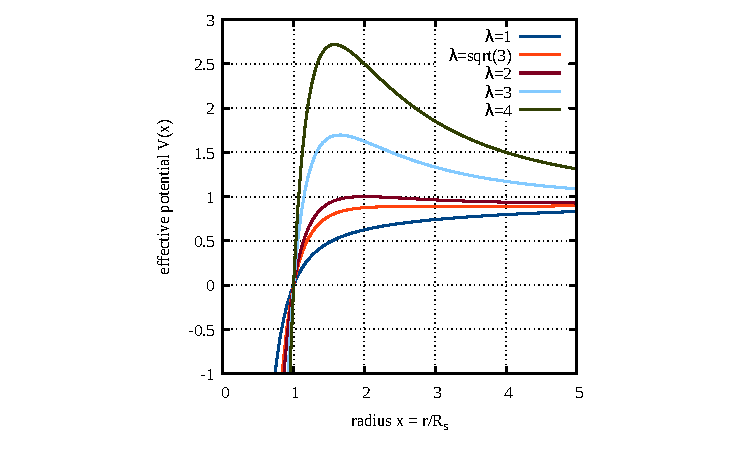
\includegraphics[width=0.48\linewidth]{gfx/fig09-1}
		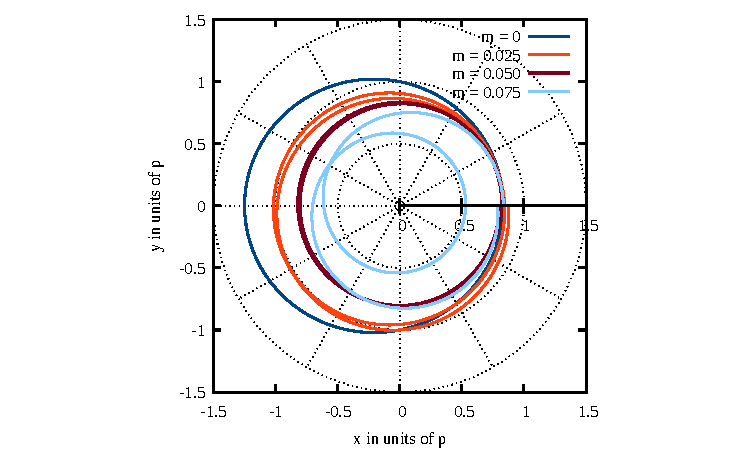
\includegraphics[width=0.48\linewidth]{gfx/fig09-2}
		\caption{\itshape Energy dependent angular-momentum barrier and non-closed elliptic orbits with perihelion shift in Schwarzschild geometry.}
		\label{fig:fig09-1}
	\end{figure}
	
	For $\lambda > \sqrt{3}, V(x=x_+)$ is minimum and $V(x=x_-)$ is maximum. This means that particles with $E\geq 1$ and $L < 2R_s$ will fall unimpededly towards $r=R_s$.\\
	\\
	Thus, In general relativity the situation is different, but only for $r$ sufficiently small. For massless particles there is always a barrier (except
	for $L = 0$, for which the potential vanishes identically), but a sufficiently energetic photon
	will nevertheless go over the barrier and be dragged inexorably down to the center. At the top
	of the barrier there are unstable circular orbits. For massive particles there are once again different regimes depending on the angular
	momentum. Thus $r=6GM$ is the smallest possible radius of a stable
	circular orbit in the Schwarzschild metric. There are also unbound orbits, which come in
	from infinity and turn around, and bound but noncircular ones, which oscillate around the
	stable circular radius. Note that such orbits, which would describe exact conic sections in
	Newtonian gravity, will not do so in GR, although we would have to solve the equation for
	dφ/dt to demonstrate it. Finally, there are orbits which come in from infinity and continue
	all the way in to $r = 0$; this can happen either if the energy is higher than the barrier, or for
	$L < \sqrt{12}GM$, when the barrier goes away entirely.\\
	We have therefore found that the Schwarzschild solution possesses stable circular orbits
	for $r > 6GM$ and unstable circular orbits for $3GM < r < 6GM$. It’s important to remember
	that these are only the geodesics; there is nothing to stop an accelerating particle from
	dipping below $r = 3GM$ and emerging, as long as it stays beyond $r = 2GM$.
	\subsection{Perihelion shift}
	The perihelion is the nearest point in the orbit, while the aphelion is the farthest. One therefore has $u^\prime=0$ and $u=u_+$ at the perihelion, since when $u$ is maximally large, then $r$ is maximally small.
		The precession of perihelia reflects the fact that noncircular orbits are
		not closed ellipses; to a good approximation they are ellipses which precess, describing a
		flower pattern.\\
		\marginpar{The
			observed value is $5601 arcsecs/100 yrs$. However, much of that is due to the precession
			of equinoxes in our geocentric coordinate system; $5025 arcsecs/100 yrs$, to be precise. The
			gravitational perturbations of the other planets contribute an additional $532 arcsecs/100 yrs$,
			leaving $43 arcsecs/100 yrs$ to be explained by GR}
		The treatment of the Kepler problem in CM shows that closed orbits in the Newtonian limit are given by
		\begin{equation}
		u_0 (p) = \frac{1}{p} (1+e \cos \varphi), \quad p=\frac{L^2}{m}=a(1-e^2).
		\end{equation}
		Assuming that the perturbations $3mu^2$ in the e.o.m. is small, we can approximate $3mu \approx 3mu_0$. The solution of the resulting equation is given by particular solutions to driven harmonic oscillator
		\begin{equation}
		u''+u= \left\{\begin{array}{lr}
		A & u_1=A\\
		B \cos \varphi & u_2 = \frac{B}{2} \varphi \sin \varphi\\
		C \cos^2\varphi & u_3 =\frac{C}{2}(1-1/3 \cos^2\varphi)
		\end{array}\right\}
		\end{equation}
		\begin{mybox}{Orbits in the Schwarzschild spacetime}
			Since the unperturbed equation $u''+u=\frac{m}{L^2}$ has the Keplerian solution $u=u_0$, the complete solution is thus the sum
			\begin{align}
				u=u_0+u_1+u_2+u_3&=\frac{1}{p} (1+e \cos \varphi) + \frac{3m}{p^2} \left[1+e \varphi \sin \varphi \right.\nonumber \\
				&\left.  + \frac{e^2}{2} (1-1/3 \cos^2\varphi)\right].
			\end{align}
		\end{mybox}
		$u'|_{\mathrm{perihelion}} = 0= \frac{\md u}{\md \varphi}$ ? $\varphi =0$ is one solution for the perihelion since $u_0$ was constructed like this. What is the next perihelion though after $\varphi = 2 \pi + \delta \varphi$?
		\begin{mybox}{Perihelion shift in the Schwarzschild metric}
			\begin{equation}
			\frac{\md u}{\md \varphi}|_{\varphi = 2 \pi + \delta \varphi} \stackrel{!}{=}0 \; \Rightarrow\; \delta \varphi \approx \frac{3 \pi R_s}{a(1-e^2)} \approx 43''
			\end{equation}
			per century for Mercury's orbit, which reproduces the measurement extremely well.
		\end{mybox}
		\subsubsection{Remark by Weinberg}
		Let $r_+$ and $r_-$ denote the aphelion and perihelion respectively, i.e. $r_{\pm} = (1 \pm e)a$. The change in $\varphi$ as $r$ decreases from $r_+$ to $r_-$ is the same as the change in $\varphi$ as $r$ increases from $r_-$ to $r_+$, so the total change in $\varphi$ per revolution is $2 \abs{\varphi(r_+)-\varphi(r_-)}$. This would equal $2\pi$ if the orbit was a closed ellipse, so in general the orbit precesses in each revolution by an angle
		\begin{equation}
		\Delta \varphi = 2 \abs{\varphi(r_+)-\varphi(r_-)} - 2\pi.
		\end{equation}
		As further remarked under light deflection, we should ask ourselves what the predicted value of $\Delta \varphi$ means. This is not a scattering experiment like the deflection of light by the sun; here we are dealing with an object that never gets out to infinity where the metric is Minkowskian. In practice, these fine points do not really matter, because the precession is cumulative.
		
		
		
		
		
		
		
		\subsection{Light deflection}
		\marginpar{Shapiro delay comes about since light does not travel in a straight line, such that there is a delay of travel time if light passes through a gravitational potential.}
		Repeating the discussion for the effective potential of light rays yields the orbital eq. for light rays in the Schwarzschild space-time:
		\begin{mybox}{E.o.m. of light rays in the Schwarzschild space-time}
			Light rays (null geodesics) in the Schwarzschild space-time follow the orbital equation
			\begin{equation}
			u''+u= 3mu^2.
			\end{equation}
		\end{mybox}
		Again, the correction $3mu^2$ is very small in our solar system and can be treated perturbatively,\\
		$\Rightarrow$ Solution of $u ''+u=0$ is a straight line in polar coordinates $u_0 = \frac{\sin  \varphi}{b}$,
		which is then shifted by the gravitational attraction of the point mass represented by $3mu^2\Rightarrow$ $3mu^2\approx 3mu^2_0$ lowest order perturbative solution
		\begin{equation}
		u=u_0+u_1 = \frac{\sin \varphi}{b} + \frac{3m}{b^2} - \frac{3m}{2 b^2} \left(1- 1/3 \cos^2\varphi\right).
		\end{equation}
		\begin{mybox}{Light deflection in the Schwarzschild metric}
			For $b$ at $\varphi=\frac{\pi}{2}$, we have a light ray coming from the left at large distances.\\
			Deflection angle for light rays is then given by
			\begin{equation}
			\alpha = 2 |\varphi| \approx \frac{4m}{b} = 2 \frac{R_s}{b} \approx 1.74 ''\qquad \mathrm{for \; sun}.
			\end{equation}
		\end{mybox}
		\begin{figure}
			\centering
			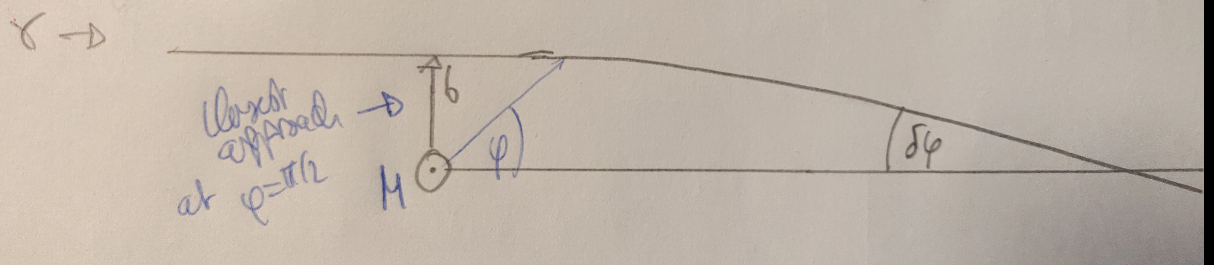
\includegraphics[width=0.7\linewidth]{gfx/LightdeflectionSchwarzschild}
			\caption{\itshape Deflection of light rays due to the gravitational effect of a mass at the centre.}
			\label{fig:lightdeflectionschwarzschild}
		\end{figure}
		
		\subsubsection{Remark by Weinberg}
		\emph{Whenever we obtain a prediction from GR the questions always arises whether the result obtained really refers to an objective physical measurement or whether it has folded into ait arbitrary subjective elements dependent on our choice of coordinate system}. Fortunately, the answer is here quite simple, for this is really a \emph{scattering} experiment. \\
		Another conceptual difficulty that may arise here has to do with our treatment of the photon as a quantum of light moving as would any other particle that happened to have a velocity close to $c$. Actually, no use is being made of QM. The wavelength of light is so small compared with the scale of the solar gravitational field that at any point in this field we can erect a locally inertial coordinate system that covers a huge number of wavelengths. The Principle of Equivalence tells us that in such a coordinate system light behaves as it does in gravitation - free empty space, and since the wavelength is so small, this means that diffraction is negligible and each element of a wave front moves in a straight line at unit velocity.
		
		
		\subsection{Redshift in Schwarzschild Spacetime}
		The gravitational redshift, as we have seen, is another effect which is present in the weak
		field limit, and in fact will be predicted by any theory of gravity which obeys the Principle
		of Equivalence. However, this only applies to small enough regions of spacetime; over larger
		distances, the exact amount of redshift will depend on the metric, and thus on the theory
		under question. It is therefore worth computing the redshift in the Schwarzschild geometry.
		We consider two observers who are not moving on geodesics, but are stuck at fixed spatial
		coordinate values $(r_1 , θ_1 , φ_1 )$ and $(r_2 , θ_2 , φ_2 )$. According to \ref{eq:Schwarzschildmetric}, the proper time of observer
		$i$ will be related to the coordinate time $t$ by
		\begin{equation}
		\frac{\md \tau_i}{\md t} = \sqrt{1-\frac{2 M \mathcal{G}}{r_i}}.
		\end{equation}
		Suppose that the observer $O_1$ emits a light pulse which travels to the observer $O_2$ , such that
		$O_1$ measures the time between two successive crests of the light wave to be $∆τ_1$ . Each crest
		follows the same path to $O_2$ , except that they are separated by a coordinate time $\Delta t$.
		This separation in coordinate time does not change along the photon trajectories, but the
		second observer measures a time between successive crests given by
		\begin{equation}
		\Delta \tau_2 = \sqrt{1-\frac{2 M \mathcal{G}}{r_2}} \Delta t = \sqrt{\frac{1-2 \mG M/r_2}{1-2 \mG M/r_1}} \Delta \tau_1.
		\end{equation}
		Since these intervals $∆τ_i$ measure the proper time between two crests of an electromagnetic
		wave, the observed frequencies will be related by
		\begin{equation}
		\label{eq:redshiftSchwarzschild}
		\frac{\omega_2}{\omega_1} = \frac{\Delta \tau_1}{\Delta \tau_2} \stackrel{r \gg 2 \mG M}{\approx} =1 -\frac{\mG M}{r_1} + \frac{\mG M}{r_2} = 1+\Phi_1 -\Phi_2.
		\end{equation}
		This tells us that the frequency goes down as Φ increases, which happens as we climb out
		of a gravitational field; thus, a redshift.
		
		
		
		
		
		
		
		
		
		
		
		
		
		
		
		
		
		
		
		
		


\newpage
\section{Black Holes}
\subsection{Schwarzschild Black Holes}
A Schwarzschild black hole or \emph{static} black hole is a black hole that has neither electric charge nor angular momentum. A Schwarzschild black hole is described by the Schwarzschild metric, and cannot be distinguished form any other Schwarzschild black hole except by its mass. The Schwarzschild black hole is characterized by a surrounding spherical boundary, called the \emph{event horizon}, which is situated at the Schwarzschild radius. The boundary is not a physical surface, and if a person fell through the event horizon (before being torn apart by tidal forces), they would not notice any physical surface at that position; it is a mathematical surface defining black hole properties. Any non-rotating and non-charged mass that is smaller than its Schwarzschild radius forms a black hole.\\
\\
The \emph{coordinate singularity} at $r=R_s$ divides the Schwarzschild coordinates in two disconnected patches. The exterior Schwarzschild solution with $r>R_s$ is the one that is related to the gravitational fields of stars and planets. The interior Schwarzschild solution with $0 \leq 0 < R_s$, which contains the singularity at $r=0$, is completely separated from the outer patch by the coordinate singularity at $r=R_s$. Using \emph{different coordinates}, one can relate the two patches as the singularity at $r=R_s$ vanishes.\\
The case $r=0$ is different. If one asks that the solution be valid for all $r$ one runs into a \emph{physical singularity}, or \emph{gravitational singularity} at the origin. This singularity is independent of coordinates as one can check from tensor invariants. At $r=0$ the curvature becomes infinite, indicating the presence of a singularity. At this point the metric, and spacetime, itself is no longer well-defined.\\
\\
The solution, i.e. the Schwarzschild black hole, for $r>0$ has bizarre properties. For $r<R_s$, the Schwarzschild radial coordinate $r$ becomes timelike and the time coordinate $t$ becomes spacelike. A curve at constant $r$ is no longer a possible world line of a particle or observer, not even if a force is exerted to try to keep it there. This occurs because spacetime has been curved so much that the direction of cause and effect (the particle's future light cone) points into the singularity. The event horizon represents the point past which no light can no longer escape the gravitational field. Any physical object whose radius $R$ becomes $R \leq R_s$ will undergo gravitational collapse and become a black hole.
\\
\\
How do you check for true singularities ?\\
We have a true singularity when the curvaure becomes infinite. The curvature is
measured by the Riemann tensor, and it is hard to say when a tensor becomes infinite, since
its components are coordinate-dependent. But from the curvature we can construct various
scalar quantities, and since scalars are coordinate-independent it will be meaningful to say
that they become infinite. This simplest such scalar is the Ricci scalar $\mathcal{R} = g_{μν} R\munu$ , but we
can also construct higher-order scalars such as $R\munu R^{μν} $ and
so on. If any of these scalars (not necessarily all of them) go to infinity as we approach some
point, we will regard that point as a singularity of the curvature. We should also check that
the point is not “infinitely far away”; that is, that it can be reached by travelling a finite
distance along a curve. See further under penrose-hawking singularity theorems \ref{subsec:HawkingPenroseSingularity}. E.g. for the Schwarzschild solution we find the true singularity to be at $r=0$ since
\begin{equation}
	\bar{R}^{\mu \nu \sigma \tau}\bar{R}_{\quad \quad \mu \nu  \sigma \tau} =\frac{12 \mathcal{G}^2 M^2}{r^6}.
\end{equation}
\subsubsection{The coordinate singularity at $r=2m$}
Consider an observer freely-falling into the centre of the black hole along a radial orbit (i.e $\dot{\phi} =0 \Rightarrow L=0$). From the e.o.m.
\begin{equation}
	\left(\frac{\md r}{\md \tau}\right)^2 + \left(1-\frac{2m}{r}\right) = E^2,
\end{equation}
one finds that the centre $r=0$ is reached after the \emph{finite proper time} (time measured by a clock moving along the same world line with the observer/test particle)
\begin{equation}
	\tau_0 = \pi \sqrt{\frac{R^3}{8 m} }< \infty.
\end{equation}
This indicates that the observer falls freely from rest at $r=R$ within finite time "through" the singularity at $r=2m$ without encountering a problem.\\
In contrast to this observation, switch to the \emph{coordinate time} $t$ (measured by a stationary clock located infinitely far from the massive body).
The free-fall coordinate time to the centre of a black hole solving the e.o.m. with $t$ instead of $\tau$ and using the tortoise radius, we find
\begin{equation}
	r = 2m+r_0 e^{-\frac{t}{2m}},
\end{equation}
showing that the Schwarzschild radius is only reached after \emph{infinitely} long coordinate time. This is equivalent to the light cone closing up as it approaches the event horizon, i.e. light ray doesn't seem to get to event horizon in coordinate time plane $(r,t)$. Compare to redshift formula \ref{eq:redshiftSchwarzschild}, where this already comes apparent as well, since as in falling astronauts approach $r = 2\mG M$, any
fixed interval $∆τ_1$ of their proper time corresponds to a longer and longer interval $∆τ_2$ from
our point of view, this continues forever. \\
\\
The \emph{tortoise coordinate} is defined as 
\begin{equation}
	r'= r- 2 m \ln{\left|\frac{r}{2m} -1\right|},
\end{equation}
and it approaches $-\infty$  as $r\rightarrow 2m$. When some probe (such as a light ray or an observer) approaches a black hole event horizon, its Schwarzschild time coordinate grows infinite. The outgoing null rays in this coordinate system have an infinite change in $t$ on travelling out from the horizon. The tortoise coordinate is intended to grow infinite at the appropriate rate such as to cancel out this singular behaviour in coordinate systems constructed from it.\\ \\
The increase in the time coordinate to infinity as one approaches the event horizon is why information could never be received back from any probe that is sent through such an event horizon. This is despite the fact that the probe itself can nonetheless travel past the horizon. It is also why the space-time metric of the black hole, when expressed in Schwarzschild coordinates, becomes singular at the horizon - and thereby fails to be able to fully chart the trajectory of an infalling probe.
\\
\\ For radial light rays one finds 
\begin{equation}
	\frac{\md r}{\md t} = \pm \left(1-\frac{2m}{r}\right), 
\end{equation}
suggesting that the light cones become infinitely narrow as $r \rightarrow 2m +$.
\\
\\
Problems on the horizon:\\
These  results appear confusing: While a freely falling observer reaches the Schwarzschild radius and even the centre of the Schwarzschild spacetime after finite proper time, the coordinate time becomes infinite even for reaching the Schwarzschild radius, and the flattening of the light cones as one approaches the Schwarzschild radius is entirely unwanted because causality cannot be assessed when the light cone degenerates to a line.
\\
\\
In coordinate time, the astronaut never reaches $r=R_s \Rightarrow$ shows that something is wrong with $r=2m \Rightarrow$ coordinate singularity.
$G_{\mu \nu}, R^a_b, \mathcal{R}$ are all defined at $r=R_s \Rightarrow$ not a prolem of the spacetime but of our choice of coordinates, i.e. of the Schwarzschild tetrad.

\subsubsection{The Kruskal continuation}
The Kruskal-Szekeres coordinates are a coordinate system for the Schwarzschild geometry for a black hole. These coordinates have the advantage that they cover the entire spacetime manifold of the maximally extended Schwarzschild solution and are well-behaved everywhere outside the physical singularity. These are coordinates in which the light-cone stays Minkowskian like $X$ all the time by construction, independent of motion.
\marginpar{The light cone itself is invariant, but in some coordinates you may not see this properly.}
\begin{mybox}{Kruskal coordinates}
	The Kruskal coordinates $(t,r) \mapsto (v,u)$ are constructed such that the light cones remain the same everywhere:
	\begin{equation}
		g = -f^2(u,v) (\md v^2 -\md u^2) + r^2 \md \Omega^2,
	\end{equation}
	such that for a light ray
	\begin{equation}
		\md s= 0 \quad \Rightarrow \quad \left(\frac{\md u}{\md v}\right)^2 =1 \; \Leftrightarrow \; \mathrm{Minkowskian \; lightcone.}
	\end{equation}
	Solving the resulting equations and applying physical boundary conditions of our Schwarzschild spacetime yields
	\begin{align}
		u &= \sqrt{\frac{r}{2m} -1 } e^{\frac{r}{4m}} \cosh{\frac{t}{4m}}, \\
		v &= \sqrt{\frac{r}{2m} -1} e^{\frac{r}{4m}} \sinh{\frac{t}{4m}}, \\
		f^2 &= \frac{32 m^3}{r} e^{- \frac{r}{2m}}.
	\end{align}
\end{mybox}
Coordinate transformation recipe:\\
\begin{equation}
	(t,r,\vartheta\varphi) \mapsto (v,u,\vartheta,\varphi) \, \Rightarrow \, (\mathcal{J}^{\alpha}_{\beta}) = \begin{pmatrix}
	\partial_t v & \partial_tu & 0&0\\
	\partial_r v & \partial_r u &0&0 \\
	0&0&1&0\\
	0&0&0&1\\
	\end{pmatrix}
\end{equation}
with $(\tilde{\mathcal{J}} ) = \frac{\partial(v,u)}{\partial (t,r)}$. Then the new metric reads
\begin{equation}
	\tilde{g} = \mathrm{diag}\left(-f^2,f^2,r^2,r^2 \sin^2\vartheta\right),
\end{equation}
and is transformed into the metric in original coordinates by

\begin{equation}
	g = \mathcal{J} \tilde{g} \mathcal{J}^T.
\end{equation}

\subsubsection{Physical meaning of the Kruskal coordinates}
We can maximally extend the Kruskal coordinates to $r \in [0,\infty)$ by $\sqrt{\frac{r}{2m} -1} \mapsto\sqrt{|\frac{r}{2m} -1|}$ due to many sign choices along the way of the derivation.\\
A static observer inside the Schwarzschild radius is also not possible anymore, since the radial-coordinate becomes time-like at $r<R_s \Rightarrow$ global Killing vector field is lost.\\
\begin{mybox}{Non-static interior of the Schwarzschild horizon}
	The Killing vector field $K=\partial_t$ for the Schwarzschild spacetime outside $r=2m$ becomes space-like for $r<2m$, which means that the spacetime cannot be static any more inside the Schwarzschild radius.
\end{mybox}
Domains of the the Kruskal spacetime:\\
Region $I$ and $III$ are asymptotically flat regions, $II$ is the interior of the black hole. Once
anything travels from region $I$ into $II$, it can never return. In fact, every future-directed path
in region $II$ ends up hitting the singularity at $r = 0$; once you enter the event horizon, you are
utterly doomed. This is worth stressing; not only can you not escape back to region $I$, you
cannot even stop yourself from moving in the direction of decreasing $r$, since this is simply
the timelike direction. Thus you can no more stop moving
toward the singularity than you can stop getting older. Since proper time is maximized along
a geodesic, you will live the longest if you don’t struggle, but just relax as you approach
the singularity. Not that you will have long to relax. (Nor that the voyage will be very
relaxing; as you approach the singularity the tidal forces become infinite. As you fall toward
the singularity your feet and head will be pulled apart from each other, while your torso
is squeezed to infinitesimal thinness. \\
\\
$IV$ is a white hole.
There is a singularity in the past, out of which
the universe appears to spring. The boundary of region $III$ is sometimes called the \emph{past event horizon}, while the boundary of region $II$ is called the \emph{future event horizon}.\\
The bold hyperbolae in regions $II$ and $IV$ are the singularities. Region $IV$,
meanwhile, cannot be reached from our region $I$ either forward or backward in time (nor can
anybody from over there reach us). It is another asymptotically flat region of spacetime, a
mirror image of ours. It can be thought of as being connected to region I by a “wormhole,” a
neck-like configuration joining two distinct regions. The dashed diagonals through the origin are the event horizons. The origin (really a 2-sphere with angular coordinates suppressed) is the throat of a non-traversable wormhole joining the separate "universes" $I$ and $III$. Radial light rays remain $45$ degree diagonal lines on the Kruskal-Szekeres diagram. The thin hyperbolae are lines of constant Schwarzschild $r$ coordinate, and the thin radial rays are lines of constant $t$. You can see how the event horizon becomes a coordinate singularity where $r$ and $t$ switch roles, i.e. at the dashed diagonal lines they switch roles and there also the event horizon is.\\
The exterior of the Schwarzschild radius corresponds to the domain $u>0, |v| < u$, and its interior is bounded in the $(u,v)$-plane by the lines $u>0,|v| =u$, and $v^2- u^2 =1$, compare \ref{fig:Schwarzschildbh}. ON figure \ref{fig:Schwarzschildbh}:
\begin{enumerate}
	\item hyperbolic lines $=r$ constant,
	\item straight lines $=t$ constant at $r=2m$. 
	\item Lines  of constant $r,t$ meet $\Rightarrow$ reflects that coordinate time $t \rightarrow \infty$ at $r=2m$
	\item (I) Everything outside $r>2m$, our world
	\item (II) everything inside $r<2m$, dark blue line represents the true singularity
	\item Beyond green bold line is "white hole". Can't keep anything for itself, light in IV has to escape. White hole would thus violate thermodynamics, the $2^{nd}$ coverage of the Kruskal coordinates is thus \emph{not physical}.
\end{enumerate}
\begin{figure}[h]
	\label{fig:Schwarzschildbh}
	\centering
	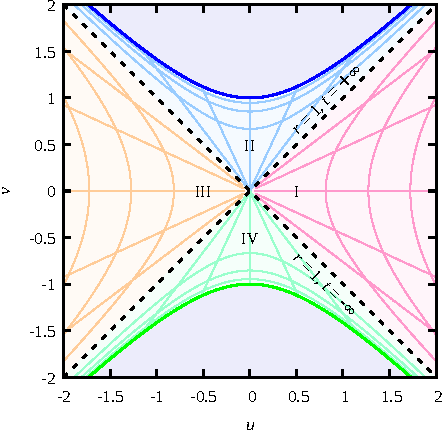
\includegraphics[width=0.8\textwidth]{gfx/fig10-2.pdf}
	\caption{\itshape Schwarzschild black hole in Kruskal coordinates, regions I \& II are double-covered by regions III \& IV.}
\end{figure}
Radial light rays propagate according to $\md s^2 =0$ or $\md v = \md u$, i.e. they are straight diagonal lines in the $(u,v)$ plane. This shows that light rays can propagate freely into the region $r<2m$, but there is no causal connection from within $r<2m$ to the outside.
\begin{mybox}{Radial light rays in Kruskal spacetime}
	The light cones are Minkowskian everywhere by construction of the Kruskal coordinates, since 
	\begin{equation*}
		\md s^2 =  0 \quad \Leftrightarrow \quad (\md u^2 - \md v^2 ) = 0 \quad \Leftrightarrow \quad \md u =\md v.
	\end{equation*}
	Radial light rays propagate according to $\md v = \md u$, i.e. they are straight diagonal lines in the
	$(u, v)$-plane. Thus, light rays can propagate freely into the region $II$ with $r < 2m$ from the outside
	region $I$, but there is no causal connection from within region $II$ with $r < 2m$ to the outside
	region I.
\end{mybox}
Now if you draw a worldline from region I going into region II it becomes obvious that it crosses the horizon in finite proper time and, more importantly, the past light-cone of the event where it hits the singularity cannot possibly contain the whole spacetime. So the short answer to the question is no, someone falling into a black hole does not see the end of the universe. Compare also
\begin{figure}[h!]
	\centering
	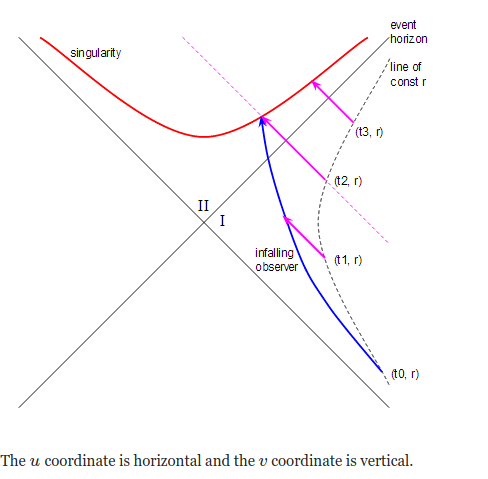
\includegraphics[width=0.7\linewidth]{gfx/kruskalszekerescoordInfallingObs}
	\caption{}
	\label{fig:kruskalszekerescoordinfallingobs}
\end{figure}
The problem with these coordinates is that they are highly unintuitive. A displacement in $u$ or $v$ doesn't correspond to any simple physical quantity, unlike a displacement in the usual radial coordinate $r$ or time coordinate $t$. Nevertheless the KS coordinates simplify things drastically as follows:
\\
In these coordinates constant $r$ is a hyperbola as shown by the dashed line. The event horizon is the solid $45°$ line. You can sort of think as $t$ increasing as you move up - it does, though not in a linear way. The singularity is the red hyperbola (this is a spacetime diagram remember, so the singularity is a curve not a point). The region I've labelled $I$ is the exterior of the black hole and the region I've labelled $II$ is the region inside the event horizon. Ignore the region of the diagram to the bottom left as it isn't relevant to my question.
\\
Finally, the key feature that makes it possible to answer my question is that all radial ingoing light rays are straight $45°$ lines running from bottom right to top left. I've drawn several such light rays as magenta lines.\\

Now we can answer my question. We start with a rocket hovering at a constant distance away from the black hole, which is represented by the black dashed hyperbola of constant $r$ (as I mentioned above you can sort of think about time increasing as you move up). At time $t0$ our observer leaves the rocket and starts falling towards the black hole. The blue line shows the trajectory followed by the observer. The observer hits the singularity at the point where the blue and red lines meet.

At time $t1$ the rocket shines a light ray at the infalling observer. The light ray, travelling at $45°$, reaches the observer before they cross the event horizon - so far so good. At time $t2$ the rocket shines a second light ray at the observer, and this light ray reaches the observer just as they hit the singularity. At time $t3$ the rocket shines a third light ray into the black hole, but this doesn't reach the observer because the observer has already hit the singularity and no longer exists. That means the observer never sees the light ray released at time $t3$. The observer sees any light ray released between $t0$ and $t2$, but doesn't see any light ray released after $t2$. So the dashed magenta line marks the boundary between light rays the observer can see and ones they can't.\\

And there is the answer to my question. The observer does not see the end of the universe because the last light ray they see is the one released at time $t2$.




















\subsubsection{Eddington-Finkelstein coordinates}
In general relativity, Eddington–Finkelstein coordinates are a pair of coordinate systems for a Schwarzschild geometry (i.e. a spherically symmetric black hole) which are adapted to radial null geodesics. Null geodesics are the worldlines of photons; radial ones are those that are moving directly towards or away from the central mass. In these coordinate systems, outward (inward) traveling radial light rays (which each follow a null geodesic) define the surfaces of constant "time", while the radial coordinate is the usual area coordinate so that the surfaces of rotation symmetry have an area of $4\pi r^2$. One advantage of this coordinate system is that it shows that the apparent singularity at the Schwarzschild radius is only a coordinate singularity and is not a true physical singularity. \\
\\
We perform the coordinate transform to the tortoise time
\begin{equation}
	(r,\vartheta,\varphi), t \mapsto t', \; t = t' - 2 m \ln{\left[\pm \frac{r}{2m} \mp 1 \right]} \; \Rightarrow \; \left\{\begin{array}{lr}
	\mathrm{upper \, sign}, & \text{for } r\geq 2m\\
	\mathrm{lower \, sign}, & \text{for } r < 2m\\
	\end{array}\right\},
\end{equation}
which yields the  line element in Eddington-Finkelstein coordinates
\todo{Insert line element here}
where the metric acquires off-diagonal elements such that it no longer
depends on $t'$ and $r$ separately.\\
\\
\begin{mybox}{Light cones in Eddington-Finkelstein coordinates}
	For radial light rays we have $\md \Omega^2 = 0, \md s =0$ implying that $\md r = - \md t'$.
	Light cones in Eddington-Finkelstein coordinates are thus defined either by
	\begin{equation}
	\label{eq:edfinklightcone}
	\frac{\md r}{\md t'} = -1 \; \Rightarrow r = -t'+ const.
	\end{equation}
or by
\begin{equation}
	\frac{\md r}{\md t'} = \frac{r-2m}{r+2m}
\end{equation}
This shows that $\md r /\md t' \rightarrow −1$ for $r \rightarrow0, \md r/\md t' = 0$ for $r = 2m$, and
	$\md r/\md t'= 1$ for $r \rightarrow \infty$. Due to the vanishing derivative of $r$ with respect
	to $t'$ at $r = 2m$, geodesics cannot cross the Schwarzschild radius from
	inside, but they can from outside because of \ref{eq:edfinklightcone}.\\
	Thus, at at $r=R_s$, the light cone changes as $X\mapsto + \Rightarrow$ light ray doesn't propagate any more at $r=R_s$ in the sense that they wrap around the black hole infinitely. As $r \rightarrow 2m + \rightarrow 0+$, causality hence changes.
\end{mybox}

\todo{Include figure of eddington finkelstein lightcones}
\begin{figure}[h!]
	\centering
	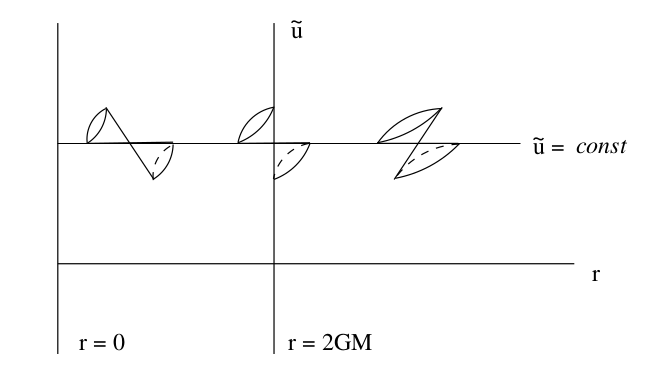
\includegraphics[width=0.7\linewidth]{gfx/eddingtonFinkelsteinLightcone}
	\caption{}
	\label{fig:eddingtonfinkelsteinlightcone}
\end{figure}

We can therefore see what has happened: in this coordinate system the light cones remain
well-behaved at $r = 2\mG M$, and this surface is at a finite coordinate value. There is no
problem in tracing the paths of null or timelike particles past the surface. On the other
hand, something interesting is certainly going on. Although the light cones don’t close up,
they do tilt over, such that for $r < 2GM$ all future-directed paths are in the direction of
decreasing $r$.\\
The surface $r = 2\mG M$, while being locally perfectly regular, globally functions as a point
of no return — once a test particle dips below it, it can never come back. For this reason
$r = 2\mG M$ is known as the \emph{event horizon}; no event at $r ≤ 2\mG M$ can influence any other event at $r > 2\mG M$. Notice that the event horizon is a null surface, not a timelike one. Notice
also that since nothing can escape the event horizon, it is impossible for us to “see inside”
— thus the name \emph{black hole}












.
\subsubsection{Redshift approaching the Schwarzschild radius}
Suppose a light-emitting source (e.g. an astronaut with a torch) is falling
towards a (Schwarzschild) black hole, what does a distant observer at rest far away from the black hole see?
The astronauts' and observers' four velocity $v,u$ define local time directions. The local frequency projected out depends on the frame of either observer or astronaut. The redshift of the light from the
torch as seen by the observer is
\begin{equation}
	1+z = \frac{\nu_{em}}{\nu_{obs}} = \frac{\langle k,v\rangle}{\langle k,u\rangle}.
\end{equation}
The calculation is performed with the used of the retarded time $\md t_{ret} = \md t - \frac{\md r}{1-\frac{2m}{r}}$, which runs on the lightcone from astronaut to observer. Radial light rays in this coordinate cannot have a time dependence : $k \propto \partial_r$. Be careful when you read of metric components from the line element, since in the line element you get off-diagonal contributions twice ! Take half their contribution, since 
\begin{equation*}
	(\md x)^T g(\md x) = \md s^2 = (\md x)^T \begin{pmatrix}
	g_{00} &g_{ij}\\
	g_{ji} & g_{aa} \\
	\end{pmatrix}
	(\md x),
	\qquad g_{ij} \dot{x}^i \dot{x}^j + g_{ji} \dot{x}^j \dot{x}^i=2 g_{ij} \dot{x}^i \dot{x}^j.
\end{equation*}
\\
A calculation shows that the astronaut’s redshift
\begin{equation}
	1+z = e^{\frac{t}{2m} -2}
\end{equation}
grows exponentially to infinity as she approaches the Schwarzschild radius. This resolves the apparent contradiction that, while the astronaut has
long reached the singularity as measured by her own watch, the distant
observer never even sees her reach the Schwarzschild radius: The signal
of the astronaut’s passing the Schwarzschild radius is infinitely delayed
and thus never reaches the distant observer.\\
The astronaut is in free fall, there is no gravity. She reaches $r=0$ instantly without delay. Observer never sees astronaut arriving at $r=R_s$, since the signal of astronaut is infinitely delayed as it is infinitely redshifted and since she reaches $r=R_s$ only at $t= \infty$ from our POV.
Paradox is not there. Signal simply never reaches the observer, even though the astronaut already entered $r< R_s$. For us it only occurs at $t=\infty$ as seen from our watch outside of black hole.
\subsubsection{Penrose (or Carter-Penrose,or conformal) diagram  - TO DO}
The idea is to do a conformal transformation which brings the entire
manifold onto a compact region such that we can fit the spacetime on a piece of paper, c.f. p. 192 caroll.\\
\\
Once again the Penrose diagrams for these spacetimes don’t really tell us anything we
didn’t already know; their usefulness will become evident when we consider more general
black holes. In principle there could be a wide variety of types of black holes, depending on
the process by which they were formed. Surprisingly, however, this turns out not to be the
case; no matter how a black hole is formed, it settles down (fairly quickly) into a state which
is characterized only by the mass, charge, and angular momentum. This property, which
must be demonstrated individually for the various types of fields which one might imagine
go into the construction of the hole, is often stated as “\emph{black holes have no hair}.”
\newpage

\subsection{Charged, Rotating Black Holes}
\subsubsection{The Reissner-Nordström solution}
The Reissner–Nordström metric is a static solution to the Einstein field equations, which corresponds to the gravitational field of a charged, non-rotating, spherically symmetric body of mass M. Now we are no longer in vacuum, since the hole will have a non-zero electromagnetic
field, which in turn acts as a source of energy-momentum.First, we consider a static, axially-symmetric solution of Einstein’s
equations in the presence of an electromagnetic charge $q$ at the origin of
the Schwarzschild coordinates, i.e. at $ r = 0$. The electromagnetic field
will then also be static and axially symmetric. The axial symmetry implies that the charge won't move, hence no $B$-field is generated and the spatial symmetry of the Schwarzschild solution is retained. We can therefore simply add the energy-momentum tensor due to the presence of the charge to the vacuum Einstein field equations for the Schwarzschild black hole. Due to the radial symmetry, the only non-vanishing component of the Faraday form is $F_{01}  = \frac{q}{r^2}$, such that the energy-momentum tensor of the electromagnetic field is readily available in the Schwarzschild tetrad. Note that the Faraday form suffices the homogeneous and inhomogeneous (in vacuum) Maxwell equations by construction.
Gravity coupled to the electromagnetic field is described by the Einstein-Maxwell
action
\begin{equation}
	S= \frac{1}{16 \pi \mG} \int \md^4 x \sqrt{-g} \left[\mathcal{R}-F\munu F^{\mu \nu} \right]
\end{equation}
where $F\munu = ∇_μ A_ν − ∇_ν A_μ$ and $A_μ$ is the electromagnetic (four-)potential. The
normalisation of the Maxwell term is such that the Coulomb force between
two charges $Q_1$ and $Q_2$ separated by a (large enough) distance $r$ is $\mG|Q_1 Q_2 |/r^2$ . This
corresponds to geometrised units of charge.\\
The field equations in this case are both
Einstein’s equations and Maxwell’s equations, thus the equations of motion derived from the variation of the Einstein-Maxwell
action are
\begin{align}
	G\munu &= 2 \left[F_{\mu \lambda} F^\lambda_{\,\; \nu} - \frac{1}{4} g\munu F_{\rho \sigma} F^{\rho \sigma} \right]\\
	\nabla_\mu F^{\mu \nu} &=0.
\end{align}
The two sets are coupled together, since the electromagnetic field strength tensor enters
Einstein’s equations through the energy-momentum tensor, while the metric enters explicitly
\marginpar{By a theorem analogous to Birkhoff’s theorem, the Reissner-Nordström solution is the unique spherically
	symmetric solution to the Einstein-Maxwell equations}
into Maxwell’s equations. They admit the spherically symmetry solution known as the Reissner-Nordström solution.
\begin{mybox}{Reissner-Nordström solution}
	Defining
	\begin{equation}
		\Delta := r^2 -2mr + Q^2, \qquad Q:= \frac{\mG q^2}{c^4}.
	\end{equation}
	we thus obtain the line element for the metric of a charged Schwarzschild black hole,
	\begin{equation}
		\md s^2 = \frac{- \Delta}{r^2} \md t^2 + \frac{r^2 \md r^2}{\Delta} + r^2 \md \Omega^2.
	\end{equation}
	This is the \emph{Reissner-Nordström solution}.
\end{mybox}
Of course, for $q = 0$, the Reissner-Nordström solution returns to the
Schwarzschild solution.
\todo{homework: set up $\mathcal{L}$, identify $V(r)$ and check what happens}
Although charged black holes with $r_q \ll  r$, with $r^2_q := \frac{\mathcal{G} q^2}{c^4}$ is a characteristic length scale, are similar to the Schwarzschild black hole, they have two horizons: the event horizon and an internal \emph{Cauchy horizon}. In physics, a Cauchy horizon is a light-like boundary of the domain of validity of a Cauchy problem (a particular boundary value problem of the theory of partial differential equations). One side of the horizon contains closed space-like geodesics and the other side contains closed time-like geodesics. The simplest example is the internal horizon of a Reissner–Nordström black hole. As with the Schwarzschild metric, the event horizons for the spacetime are located where the metric component $g^{rr}$ diverges, i.e. the equivalent to $r=2m$; that is, where
\begin{equation}
	0 =  \Delta= \frac{1}{g^{rr}} = 1- \frac{r_s}{r} + \frac{r^2_q}{r^2}, \quad r_{\pm} = \frac{1}{2} \left( r_s \pm   \sqrt{r^2_s - 4r^2_q}\right).
\end{equation}
These concentric event horizons become degenerate for $2 r_q = r_s$, which corresponds to an extremal black hole. Black holes with $2r_q > r_s$ can not exist in nature because if the charge is greater than the mass there can be no physical event horizon (the term under the square root becomes negative). Objects with a charge greater than their mass can exist in nature, but they can not collapse down to a black hole, and if they could, they would display a naked singularity. The nakedness of the singularity offends our sense of decency, as well as the \emph{cosmic censorship conjecture}, which roughly states that the gravitational collapse of physical matter
configurations will never produce a naked singularity.
\\
\\
On the true event horizons at $\Delta = (r_+ -r)(r_-r)$:\\
The singularity at $r = 0$ is a timelike line (not
a spacelike surface as in Schwarzschild). If you are an observer falling into the black hole
from far away, $r_+$ is just like $2\mG M$ in the Schwarzschild metric; at this radius $r$ switches
from being a spacelike coordinate to a timelike coordinate, and you necessarily move in the
direction of decreasing $r$. Witnesses outside the black hole also see the same phenomena
that they would outside an uncharged hole — the infalling observer is seen to move more
and more slowly, and is increasingly redshifted.\\
But the inevitable fall from $r_+$ to ever-decreasing radii only lasts until you reach the null
surface $r = r_−$ , where $r$ switches back to being a spacelike coordinate and the motion in the
direction of decreasing $r$ can be arrested. Therefore you do not have to hit the singularity
at $r = 0$; this is to be expected, since $r = 0$ is a timelike line (and therefore not necessarily
in your future). In fact you can choose either to continue on to $r = 0$, or begin to move
in the direction of increasing $r$ back through the null surface at $r = r_−$ . Then $r$ will once
again be a timelike coordinate, but with reversed orientation; you are forced to move in the
direction of increasing $r$. You will eventually be spit out past $r = r_+$ once more, which is
like emerging from a white hole into the rest of the universe. From here you can choose to
go back into the black hole — this time, a different hole than the one you entered in the
first place — and repeat the voyage as many times as you like.\\
How much of this is science, as opposed to science fiction? Probably not much. If you
think about the world as seen from an observer inside the black hole who is about to cross the
event horizon at $r_−$ , you will notice that they can look back in time to see the entire history
of the external (asymptotically flat) universe, at least as seen from the black hole. But they
see this (infinitely long) history in a finite amount of their proper time — thus, any signal
that gets to them as they approach $r_−$ is infinitely blueshifted.

\subsubsection{Kerr-Newmann solution}
The Kerr–Newman metric is the most general asymptotically flat, stationary solution of the Einstein equations in general relativity that describes the spacetime geometry in the region surrounding an electrically charged, rotating mass. It generalizes the Kerr metric (the Kerr metric or Kerr geometry describes the geometry of empty spacetime around a rotating uncharged axially-symmetric black hole with a quasispherical event horizon. ) by taking into account the field energy of an electromagnetic field, in addition to describing rotation. It is one of a large number of various different electrovacuum solutions, that is, of solutions to the Einstein equations which account for the field energy of an electromagnetic field. Such solutions do not include any electric charges other than that associated with the gravitational field, and are thus termed vacuum solutions. When a black hole is rotating, there is no analogue of Birkhoff’s theorem. This
means that, during gravitational collapse with rotating matter, we cannot use the
same reasoning as in the spherically symmetric case to argue that, on the surface of
the collapsing matter, the metric should be of the form given above. All we can say
is that, after enough time has passed and matter and spacetime have “settled down”
to equilibrium, they will be described by the Kerr-Newman solution.\\
\\
In presence of angular momentum, we expect the spherical symmetry
of the Schwarzschild solution to be broken. Instead, we expect that
the solution must be \emph{axisymmetric}, with the axis fixed by the angular
momentum. Moreover, we seek to find a stationary solution.
Then, the group $\mR \times SO(2)$ must be an isometry of the metric, where
$\mR$ represents the stationariness (can not be static since it is rotating) and $SO(2)$ the (two-dimensional) rotations
about the symmetry axis. Expressing these symmetries, there must be a
time-like Killing vector field $k$ and another Killing vector field $m$ which
is tangential to the orbits of $SO(2)$. We therefore have one Killing field for the stationariness and one for the axial symmetry.
These two Killing vector fields span the tangent spaces of the two-dimensional sub manifolds which are the orbits of $\mR \times SO(2)$, i.e. cylinders.
We can choose adapted coordinates $t$ and $\varphi$ such that $k = \partial_t$ and $m = \partial_{\varphi}$. The fact that $k,m$ are Killing vectors is equivalent to the fact that the metric coefficients do not depend on $t$ and $\varphi$.
\marginpar{The Kerr spacetime possesses a Killing tensor, c.f. Caroll p.208}
Then, the metric $^{(4)} g$ of four-dimensional space-time can be decomposed as
\begin{equation}
	^{(4)} g = g_{ab} (x^i) \md x^a \otimes \md x^b + g_{ij} (x^k) \md x^i \otimes \md x^j,
\end{equation}
where indices $a,b=0,1$ indicate the coordinates on the orbits of
$\mR \times SO(2)$, and indices $i, j, k = 2, 3$ the others. Note that, due to the
symmetry imposed, the remaining metric coefficients can only depend
on the coordinates $x^i$ .\\
\\
A stationary, axi-symmetric space-time $(M, g)$ can thus be foliated into
$M =  \Sigma \times \Gamma$, where $\Sigma \cong \mR \times SO(2)$ is diffeomorphic to the orbits of $\mR \times SO(2)$, and
the metric coefficients in adapted coordinates can only depend on the coordinates of $\Gamma$.
\\
\begin{figure}
		\centering
		\includegraphics[width=0.7\textwidth]{gfx/KerrNewmannSpacetime.jpg}
		\caption{\itshape Foliation of spacetime for the Kerr-Newmann solution.}
\end{figure}
We write
\begin{equation}
^{(4)}g = \sigma + g,
\end{equation}
where 
\begin{equation}
	\sigma = \sigma_{ab} (x^i) \md x^a \otimes \md x^b .
\end{equation}
The coefficients $\sigma_{ab}$ are scalar products of the two Killing vector fields $k$ and $m$,
\begin{equation}
	(\sigma_{ab}) = 
	\begin{pmatrix}
	-\langle k,k \rangle & \langle k, m \rangle\\
	\langle k,m \rangle & \langle m, m\rangle\\
	\end{pmatrix}, \quad \rho := \sqrt{-\det{\sigma}}.
\end{equation}\\
\\
Define the following auxilliary quantities
\begin{align*}
	\Delta & := r^2- 2mr + Q^2 +a^2, \quad \rho^2 := r^2 +a^2 \cos^2 \vartheta ,\\
	\Sigma^2 &:= (r^2+a^2)^2 -a^2 \Delta \sin^2 \vartheta, \\
	Q^2 &:= \frac{\mathcal{G}q^2}{c^4}, \quad a:= \frac{L}{Mc} = \frac{\mathcal{G}L}{m c^3}, \; [a]=[Q]=\mathrm{length}.	
\end{align*}
Note that $L$ and thus also $a$ describes the angular momentum of the rotating black hole.
\begin{mybox}{Kerr-Newmann solution}
	With these definitions, we can write the coefficients of the metric for a
	charged, rotating black hole in the form
	\begin{align}
		g_{tt} &=-1 + \frac{2mr -Q^2}{\rho^2} = g_{00, \mathrm{Schwarzschild}} |_{L,Q =0}\\
		g_{t\varphi} &= -\frac{2mr-Q^2}{\rho^2}  \sin^2\vartheta \\
		g_{\varphi \varphi} &= \frac{\Sigma^2}{\rho^2} \sin^2\vartheta, \quad g_{rr} = \frac{\rho^2}{\Delta}, \quad g_{\vartheta \vartheta} = \rho^2.
	\end{align}
Notice how $t,\varphi$ are coupled here in $g_{t \varphi}$, since we chose adapted coordinates $(t,\varphi)$ and since the black hole is rotating. They will have to point into direction of the Killing vector fields $k,m$ together, i.e. they describe screws in the cylinder.
\begin{align}
 g_{\mathrm{Kerr-Newmann}} |_{Q=0} &= g_{\mathrm{Kerr}}, \\
  g_{\mathrm{Kerr-Newmann}} |_{L=0} &= g_{\mathrm{Reissner-Nordström}}.
\end{align}
\end{mybox}

Any Kerr–Newman source has its rotation axis aligned with its magnetic axis. Thus, a Kerr–Newman source is different from commonly observed astronomical bodies, for which there is a substantial angle between the rotation axis and the magnetic moment. Specifically, neither the Sun, nor any of the planets in the Solar system have magnetic fields aligned with the spin axis. Thus, while the Kerr solution describes the gravitational field of the Sun and planets, the magnetic fields arise by a different process.
\begin{mybox}{Kerr metric}
The line element of the Kerr metric for an uncharged rotating black hole with angular momentum $\tilde{L}$
is given by
\begin{align}
	\label{eq:kerrmetric}
	\md s^2&= -\left(1-\frac{2mr}{\rho^2}\right) \md t^2 - \frac{4mra}{\rho^2} \sin^2 \vartheta \md t \md \varphi + \frac{\rho^2}{\Delta}\md r^2\nonumber \\
	& + ρ^2 \md\vartheta^2 + \frac{\Sigma^2}{\rho^2} sin^2 \vartheta \md φ^2,
\end{align}
with
\begin{align}
	ρ^2 &≡ r^2 + a^2 \cos^2 \vartheta,\;	∆ ≡ r^2 − 2mr + a^2 ,\nonumber \\
	Σ^2 &≡ (r^2 + a^2)^2 − a^2 ∆ \sin^2 \vartheta, \; a=\frac{\mG \tilde{L}}{mc^3}.\nonumber
\end{align}
\end{mybox}
A note on the singularities in the KN-solution:
\begin{enumerate}
	\item One is $\Delta=0$, the resulting equation has three distinct cases where the only physical one is $\mG^2 M^2 > a^2$, which has the two null surfaces (which turn out to be event horizons)
	\begin{equation}
		r_{\pm} = \mG M \pm \sqrt{\mG^2 M^2-a^2}.
	\end{equation}
	\item Besides the event horizons at $r_±$ , the Kerr solution also features an additional surface
	of interest. Recall that in the spherically symmetric solutions, the “timelike” Killing vector
	$k^μ = ∂_t$ actually became null on the (outer) event horizon, and spacelike inside. Analogously for Kerr yields
	 \begin{equation}
	 k_\mu k^\mu = −\frac{1}{\rho^2}	(∆ − a^2 \sin^2 θ).
	 \end{equation}
	 This does not vanish at the outer event horizon; in fact, at $r = r_+$ (where $∆ = 0$), we have
\begin{equation}
		k^2 = \frac{a^2}{\rho^2} \sin^2\theta \geq 0.
\end{equation}	
	So the Killing vector is already spacelike at the outer horizon, except at the north and south
	poles ($θ = 0$) where it is null.\\
	The locus of points where $k^\mu k_\mu = 0$ is known as the \emph{Killing
	horizon}, and is given by
\begin{equation}
	(r − \mG M)^2 = \mG^2 M^2 − a^2 \cos^2 θ ,
\end{equation}
while the outer event horizon is given by
\begin{equation}
	(r_+ − \mG M)^2 = \mG^2 M^2 − a^2.
\end{equation}
There is thus a region in between these two surfaces, known as the \emph{ergosphere}. Inside the
ergosphere, you must move in the direction of the rotation of the black hole (the $\phi$ direction);
however, you can still move towards or away from the event horizon (and there is no trouble exiting
the ergosphere).
\item True curvature singularity occurs in this spacetime at
\begin{equation}
	\rho=0 \quad \Leftrightarrow \quad r=0 \, \& \, \theta=\frac{\pi}{2}.
\end{equation}
This seems like a funny result, but remember that $r = 0$ is not a point in space, but a disk;
the set of points $r = 0, θ = π/2$ is actually the ring at the edge of this disk. The rotation
has “softened” the Schwarzschild singularity, spreading it out over a ring.\\
The region near the ring singularity has additional pathologies: closed timelike curves. Since these paths are closed, they are obviously closed time-like curves (c.f. CTC on Wikipedia). You can therefore meet yourself in the past, with all that entails.
\end{enumerate}
\vspace{1.5cm}
The vector potential of the rotating,
charged black hole is given by the 1-form
\begin{equation}
	A = - \frac{q r}{\rho^2} (\md t - a \sin^2\vartheta \md \phi), \quad F=\md A.
\end{equation} 
In the limit of large $r$, i.e. $a \ll r$, the
electric field thus becomes that of a point charge q at the origin, and the
magnetic field has a characteristic dipolar structure. From the non-vanishing (magnetic) field components
\begin{equation}
	E_r = F(e_r,e_t)=\frac{q}{r^2}, \; B_r = F(e_{\vartheta}, e_{\varphi}) = \frac{2qa}{r^3} \cos \vartheta,\; B_{\vartheta} = F(e_{\vartheta}, e_r) = \frac{q a}{r^3} \sin \vartheta,
	\end{equation}
	 one can read of the magnetic dipole moment for a sphere.
	 \begin{mybox}{Magnetic dipole moment of a charged, rotating black hole}
	 The magnetic dipole moment of a charged, rotating black holes has the
	 modulus
\begin{equation}
	\mu = qa =2 \frac{qL}{2 Mc},
\end{equation}
	 showing that its gyromagnetic moment is g = 2.
	 \end{mybox}
 \vspace{1cm}
 Interesting properties:
 \begin{enumerate}
\item 	Since the metric coefficient satisfy the following relations w.r.t. to the symmetries of the system expressed by the two Killing vector fields in adapted coordinates
	\begin{equation}
	g_{tt} = \langle k,k\rangle,\quad g_{\varphi,t} = \langle m, k\rangle, \quad g_{\varphi \varphi} = \langle m,m \rangle,
	\end{equation}
	they have an invariant meaning, which will be discussed in the following. Consider an observer on a circular orbit in equatorial plane, i.e. $\vec{L}_{BH} \parallel \vec{L}_O$, of the black hole orbiting with a uniform angular velocity $\omega$ (as seen by a distant observer). Since the black hole is rotating, the rotational direction, whether observer rotates with or against the black hole, matters a lot due to the \emph{drag of spacetime} induced by the black hole. At which radius does the four velocity of the observer become light-like $u =c?, \Leftrightarrow \langle u, u \rangle =0?$
	\begin{equation}
		\Leftrightarrow w_{\pm} = \Omega \pm \sqrt{\Omega^2 - \frac{g_{tt}}{t_{\varphi \varphi}}}.
	\end{equation}
	Note that freely-falling test particles on
	radial orbits have zero angular momentum and thus
	$\Omega$ is the frequency an observer will have on a circular orbit around the black hole if she has no angular momentum, i.e. the angular velocity solely due to the frame drag of the spacetime by the black hole. This is found by
	\begin{equation}
		0 = \langle u,m\rangle \quad \Rightarrow \quad \Omega := -\frac{g_{t\varphi}}{g_{\varphi \varphi}}.
	\end{equation}
	\begin{mybox}{What do radial orbits look like for KN-bh for distant observer ?}
		A particle that moves initially only radially towards a Kerr-Newman black hole seems like as if it
		co-rotates with the black hole the faster the closer it approaches the event horizon to observers at
		infinity due to the frame-dragging effect. Here, frame-dragging means that an inertial reference
		frame is entrained by the rotating black hole to participate in the latter’s rotation.
	\end{mybox}
	This shows that $\Omega$ is the angular
	velocity of a test particle falling freely towards the black hole on a radial
	orbit. From the outside, a particle infalling onto bh will orbit it with angular frequency $\Omega$ due to the frame-drag of the bh. How can a particle falling freely
	on a radial orbit have an angular
	velocity ? It has by the frame drag of the black hole.
	\begin{mybox}{Static limit in the Kerr spacetime}
		The minimum angular velocity $\omega_-$ vanishes if and only if
		$g_{tt} = \langle k, k \rangle = 0$, i.e. if the Killing vector field $k$ turns light-like.
		From the metric component, this is equivalent to
		\begin{equation}
			g_{tt} = 0 \; \Rightarrow \; r_0 = m + \sqrt{m^2 - Q^2 -a^2 \cos^2\vartheta}.
		\end{equation}
		The radius $r_0$ marks the static limit of Kerr space-time: for an observer
		at this radius to remain static with respect to observers at infinity
		(i.e. with respect to the “fixed stars”), she would have to move with the
		speed of light. At smaller radii, observers cannot remain static against
		the drag of the rotating black hole.
		If you get close, even if $u=c$ against the drag of the black hole, you will be seen from outside as falling onto black hole.\\
		The hypersurface defined by the static limit is time-like, which means that
		it can be crossed in both directions, in contrast to the event horizon, which can only be crossed
		to the inside. The region in between the static limit and the event horizon is the ergosphere, in
		which no observer can be prevented from following the rotation of the black hole.
	\end{mybox}
	 	\item For an observer at rest far away from the black hole and an astronaut sending signals, the redshift tends to infinity as the source approaches the static limit.
	 	\item At which radius for a distant observer doesn't it matter any more whether you orbit with or against the black hole, since frame dragging is so dominant that you are pulled away with $v=c$ anyway ? This is given by $\omega_- = \omega_+ \Leftrightarrow \Delta=0$, which describes another spherical hyper surface and a \emph{true} horizon
	 \begin{equation}
	 	r_H = m + \sqrt{m^2-Q^2- a^2}.
	 \end{equation}
	 This event horizon for the KN-bh is smaller than the Schwarzschild radius, i.e. $r_H$ plays the role of the Schwarzschild radius here, it \emph{its} the event horizon.
	 The hypersurface H is rotating with the constant angular velocity
	 \begin{equation}
	 	\Omega_H = \Omega(r_H) = \frac{a^2}{r^2_H+a^2},
	 \end{equation}
	 like a solid body.
	 \begin{figure}[h]
	 	\centering
	 	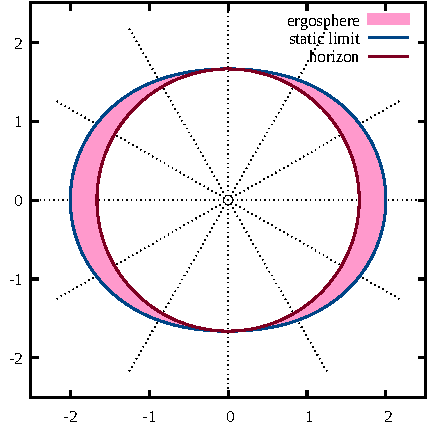
\includegraphics[width=0.7 \textwidth]{gfx/ergosphere.pdf}
	 \end{figure}
	 In the pink area between the two limits, one can in principle still escape from the black hole but can not be stationary against the outside world. The ergosphere is a region located outside a rotating black hole's outer event horizon. The ergosphere touches the event horizon at the poles of a rotating black hole and extends to a greater radius at the equator.  The equatorial (maximal) radius of an ergosphere corresponds to the Schwarzschild radius of a non-rotating black hole; the polar (minimal) radius can be as little as half the Schwarzschild radius (the radius of a non-rotating black hole) in the case that the black hole is rotating maximally (at higher rotation rates the black hole could not have formed). \\
	 \\
	 As a black hole rotates, it twists spacetime in the direction of the rotation at a speed that decreases with distance from the event horizon. This process is known as the Lense–Thirring effect or frame-dragging. By virtue of this dragging effect, an object within the ergosphere cannot appear stationary with respect to an outside observer at a great distance unless that object were to move at faster than the speed of light (an impossibility) with respect to the local spacetime. The speed necessary for such an object to appear stationary decreases at points further out from the event horizon, until at some distance the required speed is that of the speed of light. The set of all such points defines the ergosphere surface, called \emph{ergosurface}. The outer surface of the ergosphere is called the \emph{static surface or static limit}. This is because world lines change from being time-like outside the static limit to being space-like inside it. It is the speed of light that arbitrarily defines the ergosphere surface. Such a surface would appear as an oblate that is coincident with the event horizon at the pole of rotation, but at a greater distance from the event horizon at the equator. Outside this surface, space is still dragged, but at a lesser rate.
	 
	 \item Since the hypersurface $H$ is defined by the condition $∆ = 0$, its normal
	 vectors are given by
	 \begin{equation}
	 	\mathrm{grad} \Delta = \md \Delta^{\#}, \quad \md \Delta = 2(r-m) \md r.
	 \end{equation}
Thus, the norm of the normal vectors is 
\begin{equation}
 	\langle \mathrm{grad} \Delta, \mathrm{grad} \Delta \rangle = 4 g^{rr} (r-m)^2 \propto \Delta = 0
\end{equation}
on the hypersurface, showing that $H$ is a \emph{null hypersurface}. Because of this fact, the tangent space to
the null hypersurface $H$ at any of its points is orthogonal to a null vector,
and hence it does not contain time-like vectors, i.e. \textbf{you cannot cross the inner horizon $H$ ?}
\begin{mybox}{Killing horizon and ergosphere}
	The surface $H$ is called a \emph{Killing horizon}. The hypersurface defined
	by the static limit is time-like, which means that it can be crossed in
	both directions, in contrast to the horizon $H$. The region in between
	the static limit and the Killing horizon is the ergosphere, in which $k$ is
	space-like and no observer can be prevented from following the rotation
	of the black hole.
\end{mybox}
Associated to a Killing horizon is a geometrical quantity known as surface gravity, $\kappa$ . If the surface gravity vanishes, then the Killing horizon is said to be degenerate. The temperature of \emph{Hawking radiation} is related to the surface gravity $\kappa c^2$, $T_H=\frac {\hbar c\kappa }{2\pi k_{B}}$.
\item If you bend/twist spacetime too much, it breaks, gets holes and thus singularities are formed (c.f. singularity theorems by Penrose and Hawking \ref{sec:singularityHawkingPenrose}).
\item Formally, the Kerr solution is singular where $∆ = 0$, but this is a coordinate singularity.
\item Observer at static limit sends signal $\tilde{k}$ to static observer ($u=(t,\vec{0})^T$) far away:\\
	Observers at rest in a stationary space-time have four-velocities proportional to the Killing vector field $k$,
	\begin{equation}
		u \propto k, \quad u=\frac{k}{\sqrt{-\langle k,k\rangle}} = \frac{k}{\sqrt{-g_{tt}}}.
	\end{equation}
	We have seen that the projection of a Killing vector $K$ on a
	geodesic $γ$ is constant along that geodesic, $∇_{\dot{\gamma}}̇ \langle \dot{\gamma}, K\rangle = 0$. The light ray
	propagating from the source to the observer is a null geodesic with $\dot{\gamma}̇ = \tilde{k}$,
	hence
	\begin{equation}
		\nabla_{\tilde{k}} \langle \tilde{k},k\rangle =0
	\end{equation}
	and thus $\langle \tilde{k},k \rangle_0=\langle \tilde{k},k \rangle_s$. Using this we find
	\begin{align}
	1+z &= \frac{\nu_{src}}{\nu_{obs}} = \frac{\langle \tilde{k},u\rangle_{src}}{\langle \tilde{k},u\rangle_{obs}} \\
	&= \frac{\sqrt{-g_{tt}}_{obs} }{\sqrt{-g_{tt}}_{src}} \underbrace{\frac{\langle \tilde{k},k \rangle_{src}}{\langle \tilde{k},k \rangle_{obs}}}_{=1} .
	\end{align}
For an observer at rest far away from the black hole, $\langle \tilde{k},k\rangle_{obs} \approx- 1$, and the redshift becomes
\begin{equation}
	1+z \approx \frac{1}{\sqrt{-\langle \tilde{k},k\rangle_{src}}} =(- g_{tt})^{-\half}
\end{equation}
which tends to infinity as the source approaches the static limit, i.e. already at the outer horizon.\\
For a distant observer, $g_{tt} = \eta_{tt} = -1$. For the observer at static limit we further know that $\omega_- = 0 \Leftrightarrow g_{tt} \stackrel{!}{=}0$. Thus, $z\rightarrow \infty$ for source approaching the static limit. Static source here means swimming with the black hole drag. If you have proper acceleration, then $u \propto k$ is not satisfied anymore.
\item Einstein cat $\Rightarrow$ inside event horizon is region of spacetime causally disconnected from outside world; the discussed horizons are horizons \emph{against} the outside world. It is about defining the surface against whom. You are not dead as soon as $r<R_s$, you just can not communicate any more with the outside world.
\end{enumerate}
\subsubsection{Motion near a Kerr-Black Hole}
	Consider the motion of a non-charged object on a circular orbit in the equatorial plane around the black hole, i.e. $\dot{r}=0=q, \vartheta=\pi/2$.
	The Lagrangian becomes:
	\begin{equation}
		\mL = \half \left[- \left(1 - \frac{2m}{r} \right) \dot{t}^2 \underbrace{- \frac{4 m a}{r} \dot{t} \dot{\varphi}}_{=(g_{t\varphi}+g_{\varphi t}) \dot{x}^t \dot{x}^{\varphi}} + (r^2+a^2+2ma^2) \dot{\varphi}^2\right].
	\end{equation}
	Since $\dot{r}$ is a cyclic coordinate, the Euler-Lagrange equations yield a force equation which tell us where we an have a stable radial orbit:
	\begin{equation}
		\underbrace{\frac{\partial \mL}{\partial r}}_{"\frac{\partial F}{\partial r}"=0} = \frac{\md}{\md t} \frac{\partial \mL}{\partial \dot{r}}=0 ;\Rightarrow\;\frac{\partial \mL}{\partial r} = 0.
	\end{equation}
 This is equivalent to the following.
 \begin{mybox}{Kepler's third law for the KN-black hole}
 	For $\omega=\frac{\md \varphi}{\md t} = \frac{\dot{\varphi}}{\dot{t}}$ one finds two solutions of the radial equation
 	\begin{equation}
 		\omega_{\pm} = \pm \sqrt{m} \frac{1}{r^{\frac{3}{2}} \pm \sqrt{m}a}.
 	\end{equation}
 	The sign tells us that the frequency depends on whether the test particle moves with or against the rotation (i.e. with or against the induced frame drag of spacetime) of the black hole.
 \end{mybox}
Trajectories of test particles in the vicinity of a Kerr black hole look like the following figure \ref{fig:trajectorieskerrbh}.
\begin{figure}
	\centering
	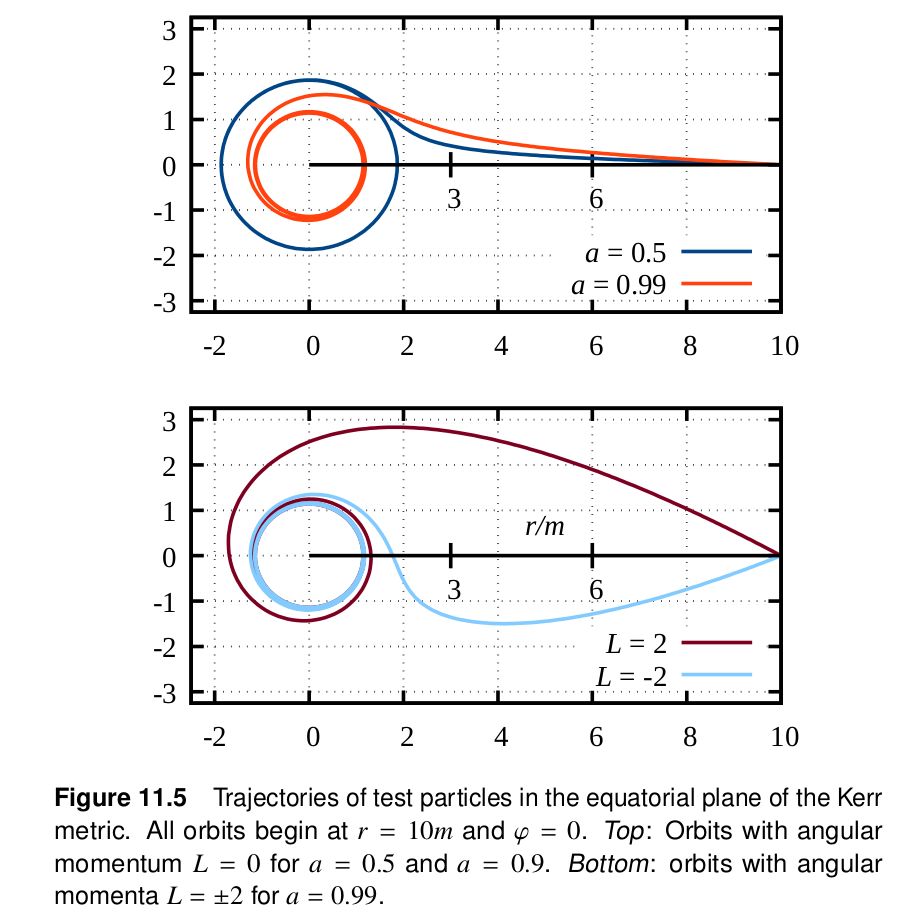
\includegraphics[width=0.7\textwidth]{gfx/TrajectoriesKerrBH}
	\caption{}
	\label{fig:trajectorieskerrbh}
\end{figure}
	
	
	\newpage
	
	\subsection{Entropy and Temperature of a Black Hole}
	Is there a violation of the second law of thermodynamics taking place by a black hole taking in object with entropy, but not giving anything back, i.e does the entropy of the Universe decrease by this ? $\rightarrow$ Assign an entropy to the BH itself.\\
	It was realised by Stephen Hawking, Roger Penrose and Demetrios
	Christodoulou that the area of a possibly charged and rotating black hole,
	defined by
	\begin{equation}
		A = 4 \pi \alpha := 4 \pi (r^2_+ + a^2), \quad r_{\pm} = m \pm \sqrt{m^2-Q^2-a^2},\, \vec{a}=\frac{\vec{L}}{M c} = \frac{\mathcal{G} \vec{L}}{c^3 m},
	\end{equation}
	cannot shrink $\Rightarrow A \equiv S ?$.\\
	\\
	This led Jacob Bekenstein (1973) to the following consideration. If $A$
	cannot shrink, it reminds of the entropy as the only other quantity known
	in physics that cannot shrink. Could the area $A$ have anything to do
	with an entropy that could be assigned to a black hole? In fact, this is
	much more plausible than it may appear at first sight. Suppose radiation
	disappears in a black hole. Without accounting for a possible entropy of
	the black hole, its entropy would be gone, violating the second law of
	thermodynamics. The same holds for gas accreted by the black hole: Its
	entropy would be removed from the outside world, leaving the entropy
	there lower than before.\\
	\\
	If, however, the increased mass of the black hole led to a suitably in-
	creased entropy of the black hole itself, this violation of the second law
	could be remedied.
	\begin{mybox}{Analogy between area and entropy}
	Any mass and angular momentum swallowed by a black hole leads to
	an increase of the area $A$, which makes it appear plausible that
	the area of a black hole might be related to its entropy
	\end{mybox}
	Try to derive an analogue to the first law of thermodynamics:\\
	Calculate all the derivatives appearing in
	 \begin{equation}
	 	\md \alpha = 2 (r_+ \md r_+ + \vec{a} \cdot \md \vec{a}), \quad \delta r:= r_+ - r_,
	 \end{equation}
	 to find
	 \begin{equation}
	 	\md m =\underbrace{ \frac{\delta r}{4 \alpha } \md \alpha}_{ \Theta\md S} +\underbrace{ \frac{r_+}{\alpha} Q \md Q + \frac{\mathcal{G}}{c^3} \frac{\vec{a}\cdot \md \vec{L}}{\alpha }}_{"Work"}
	 \end{equation}
	 where the work is work exerted on the black hole from outside world (change $\vec{L}, Q$...). This reminds of the first law of thermodynamics if we tentatively associate $m$ with the internal energy, $α$ with the entropy and the remaining
	 terms with external work. \\
	 \\
	 \marginpar{Planck units: $\lambda_{pl} = \frac{\hbar}{M_{pl} c}$ planckian compton wavelength, then the gravitational binding energy has to stabilize rest energy: $\frac{\mathcal{G}M^2_{pl}}{\lambda_{pl}} \stackrel{!}{=} M_{pl} c^2$, thus $M^2_{pl} = \frac{\hbar c}{\mathcal{G}}$, $\lambda^2_{pl} = \frac{\mathcal{G} \hbar}{c^3}$. Further, $E_{pl} = M_{pl} c^2$, i.e. $T_{pl} = \frac{E_{pl}}{k_B}$.}
	 Let us now see whether a linear relation between the entropy $S$ and the
	 area $α$ will lead to consistent results. Thus, assume $S = γα$ with some
	 constant $γ$ to be determined. Then, a change $δα$ will lead to a change
	 $δS = γδα$ in the entropy. Bekenstein showed that the minimal change of the effective area is twice
	 the squared Planck length, thus
	 \begin{equation}
	 	\delta \alpha =2 \frac{\mathcal{G}\hbar}{c^3}.
	 \end{equation}
	 On the other hand, he identified the minimal entropy change of the black
	 hole with the minimal change of the Shannon entropy, which is derived
	 from information theory and is
	 \begin{equation}
	 	S = k_B \ln 2,
	 \end{equation}
	 where the Boltzmann constant $k_B$ was inserted to arrive at conventional
	 units for the entropy. This could e.g. correspond to the minimal information loss when a single particle disappears in a black hole.
	\begin{mybox}{Bekenstein entropy }
		The Bekenstein entropy of a black hole is
		\begin{equation}
			S = \frac{\ln 2}{8  \pi } k_B \frac{c^3}{\mathcal{G} \hbar} A,
		\end{equation}
		where $A$ is the area of the black hole. This assignment was motivated by trying to save the thermodynamic laws, don't know if it is true.
	\end{mybox}
	With $E=Mc^2= \frac{m c^4}{\mathcal{G}}$, we find 
	\begin{equation}
		\frac{1}{T} = \left(\frac{\partial S}{\partial E}\right)_{V,N} = \frac{\ln 2}{2} k_B \underbrace{\left(\frac{\partial \alpha}{\partial m}\right)_{Q,L}}_{\frac{1}{\Theta}},= \ln 2 \frac{k_B \mathcal{G} M}{\hbar c^3}.
	\end{equation}
\begin{mybox}{Temperature of a Black Hole}
The analogy between the area of a black hole and entropy implies that
black holes can be assigned the temperature
\begin{equation}
	T = \frac{2}{\ln 2} \frac{\hbar c}{k_B} \Theta= \frac{2 \pi}{\ln 2} \frac{\hbar c}{k_b} \frac{\delta r}{A} = \frac{T_{pl}}{\ln 2} \left(\frac{M_{pl}}{M}\right),
\end{equation}
where the latter equality holds for an uncharged and non-rotating black hole.
\end{mybox}
	
	This result leads to a remarkable conclusions:
	\begin{enumerate}
		\item  If black holes have a
	temperature, they will radiate and thus lose energy or its mass equivalent. They can therefore evaporate.
	
	\item As the mass increases, temperature goes down. This system defies the 3rd law of thermodynamics ($S=0$ at $T=0$, since
	\begin{equation}
		T \propto \frac{1}{M}.
	\end{equation}
	Since $T ∝ M^{−1}$ and $S ∝ M^2$ , where $M$ is the black-hole mass, one has $S → ∞$ for $T → 0$, in
	gross contrast to the statement from classical thermodynamics.\\
	But there is some fundamental analogy between BH(areas) and thermodynamics.
	\item If bh has $T>0$ finite temperature, it has to radiate, it has a luminosity, this is  \emph{Hawking radiation}.\\
	The black hole thus must evaporate. The evaporation time is the slower the lower its mass.\\
	Note that $\alpha$ only does \emph{not descrease} if you neglect the loss by Hawking radiation (think of microcanonical ensemble without exterior particle exchange ??).
	
	\item $T$ is equivalent to the temperature of (Planck) spectrum of a(n) (anti-)particle whose partner anti(particle) has fallen into the bh. This can be computed by solving the corresponding QFT on a curved spacetime in the vicinity of the black hole.
	\item $S=\gamma \alpha$ is identification of the interior of bh (of which we do not and can not have any knowledge due to horizon) with the exterior world. Thus, identify processes interior with $\alpha$, which implies the use of the\emph{holographic principle} (map interior onto surface of bh), c.f. \emph{AdS/CFT correspondence}..
	 \item For a black hole of solar mass, the temperature is $T=5\times 10^{-7} \mathrm{K}$.
	 \item This analogy for $S_{BH}$ is additive w.r.t the are of the black hole, and not w.r.t the mass, since they are inverse proportional, but it has to be this way since GR is not linear, you can not superpose the gravitational effect of different masses.
\end{enumerate}
	
	
	
	
	
\section{Cosmology}
Cosmology is one of the biggest application of GR. We will therefore treat it in a separate chapter.
